\section{Évaluation de l'hypothèse de robustesse}
\label{section:4.6-HYPOTHESE-ROBUSTESSE}

	%%%
	%%% Introduction / Transition.
	%%%
	Dans les précédentes études, nous avons presque toujours analysé le \texttt{Clustering Interactif} en supposant que l'annotateur connaît parfaitement le domaine traité par le jeu de données et qu'il est capable de caractériser sans ambiguïté la similitude entre deux données issues de cet ensemble.
	Bien entendu, cette hypothèse forte n'est pas toujours vérifiée en situation réelle : l'interprétation du langage peut contenir certaines ambiguïtés, l'opérateur peut faire des erreurs d'inattention, et deux annotateurs peuvent avoir des avis contraire sur un même sujet.
	Or, comme notre méthode d'annotation est itérative, elle est a priori sensible aux dérives fonctionnement liées à ce type de contradictions.
	Dans cette section, nous nous intéressons donc à la robustesse du \texttt{Clustering Interactif} en présence d'incohérences dans les contraintes et aux moyens de les contrer.
	Pour cela, nous aimerions donc vérifier l'hypothèse suivante :
	
	%%%
	%%% Formulation des hypothèses.
	%%%
	\begin{tcolorbox}[
		title=\faVial~\textbf{Hypothèse de robustesse}~\faVial,
		colback=colorTcolorboxHypothesis!15,
		colframe=colorTcolorboxHypothesis!75,
		width=\linewidth
	]
		% Hypothèse.
		\textguillemets{\textbf{
			Au cours d'une méthodologie d'annotation basée sur le \texttt{Clustering Interactif}, il est possible d'estimer le taux d'incohérences dans les contraintes ainsi que leur impact sur les résultats de la méthode.
		}} \\
		
		% Figure.
		La \textsc{Figure~\ref{figure:4.6-HYPOTHESE-ROBUSTESSE}} illustre cette hypothèse et l'espoir de estimer l'impact de différences d'annotations sur le nombre d'itérations de la méthode.
		%
		\begin{figure}[H]  % keep [H] to be in the tcolorbox.
			\centering
			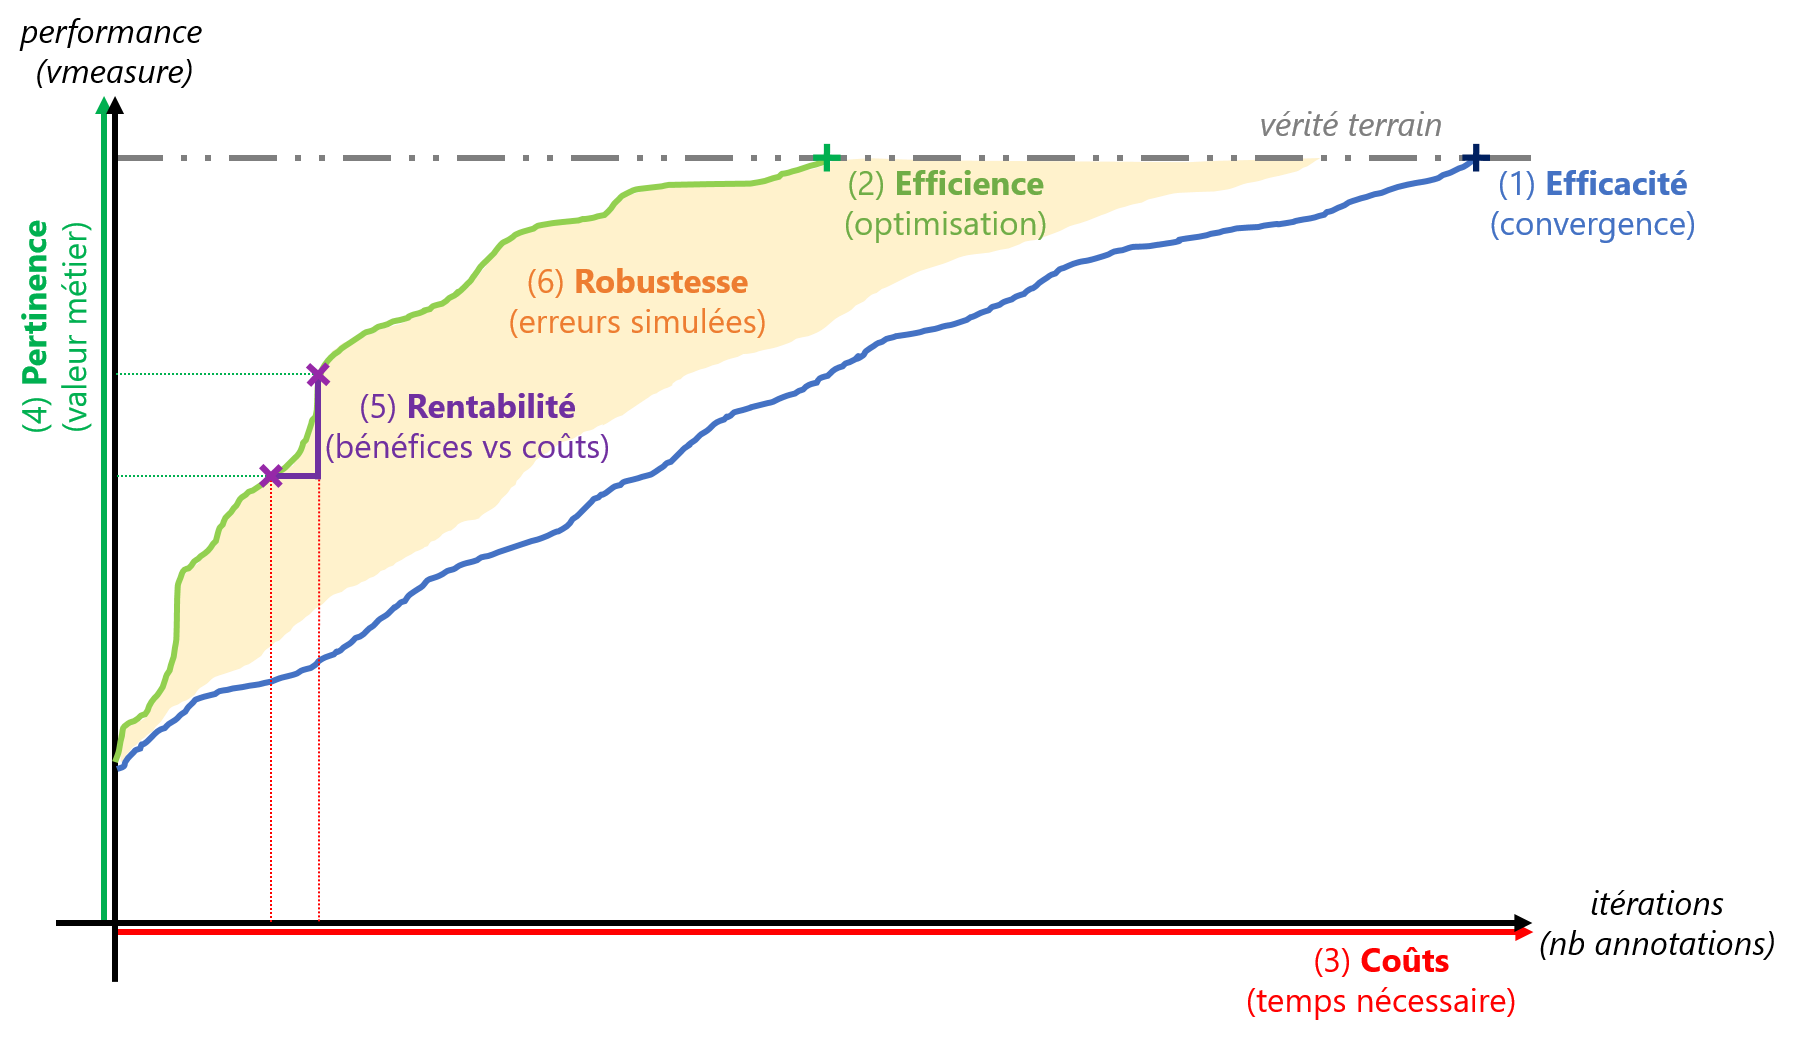
\includegraphics[width=0.95\textwidth]{figures/hypotheses-06-robustesse}
			\caption{
				Illustration des études réalisées sur le \texttt{Clustering Interactif} (\textit{étape 6/6}) en schématisant l'évolution de la pertinence (\textit{valeur métier évaluée par l'expert et exprimé en nombre de clusters}) d'une base d'apprentissage en cours de construction en fonction du coût temporel de la méthode (\textit{temps nécessaire à l'expert métier et à la machine}), ainsi que les marges d'erreurs représentant l'impact de différences d'annotation sur le nombre d'itérations nécessaire à la méthode.
			}
			\label{figure:4.6-HYPOTHESE-ROBUSTESSE}
		\end{figure}
	\end{tcolorbox}
	
	
	% Résumé des études.
	Afin de vérifier cette hypothèse, nous organisons trois expériences :
	\begin{itemize}
		\item une étude de cas d'un \textbf{score inter-annotateurs} obtenu lors d'une annotation de contraintes en situation réelle avec plusieurs opérateurs, permettant d'estimer une borne maximale du taux de désaccords d'annotation pour les autres études (cf. \textsc{Section~\ref{section:4.6.1-ETUDE-ROBUSTESSE-SCORE-ACCORD}}) ;
		\item une étude de l'\textbf{impact d'une erreur d'annotation} et de l'\textbf{intérêt de la corriger}, en simulant l'insertion d'erreurs d'annotation et en mesurant la similarité du \textit{clustering} obtenu avec la vérité terrain (cf. \textsc{Section~\ref{section:4.6.2-ETUDE-ROBUSTESSE-ERREURS-ANNOTATION-ET-CORRECTION}}) ;
		\item une étude de l'\textbf{impact de la subjectivité de l'annotation sur la divergence des résultats de \textit{clustering}}, en simulant l'insertion de différences d'annotation et en mesurant la similarité entre les \textit{clusterings} obtenus (cf. \textsc{Section~\ref{section:4.6.3-ETUDE-ROBUSTESSE-SUBJECTIVITE-ANNOTATION-ET-DIVERGENCE}}).
	\end{itemize}
		
		
	%%%
	%%% Subsection 4.6.1: Étude du score inter-annotateurs obtenu avec des opérateurs en situation réelle.
	%%%
	\subsection{Étude du score inter-annotateurs obtenu avec des opérateurs en situation réelle}
	\label{section:4.6.1-ETUDE-ROBUSTESSE-SCORE-ACCORD}
		
		% Objectif de l'expérience.
		Afin d'affiner le champ de recherche de nos futures études, nous voulons analyser le score d'accord inter-annotateurs calculé lors d'une expérience d'annotation de contraintes par plusieurs experts métiers en situation réelle.
		Pour cela, nous reprenons l'expérience de la \textsc{Section~\ref{section:4.3.1-ETUDE-COUTS-TEMPS-ANNOTATION}} visant à estimer le temps moyen d'annotation d'un lot de contraintes, et nous réutilisons ces résultats pour en estimer l'accord inter-annotateurs.
		Comme l'objectif de cette précédente étude n'était pas d'étudier la qualité des annotation, aucun guide ni aucune règles d'annotation précises n'avaient été fournies : nous espérons donc pourvoir \textbf{estimer une borne maximale grossière du désaccord entre annotateurs} lors de l'utilisation de notre méthode, permettant ainsi d'affiner notre discussion.
		
		%%% Protocole expérimental.
		\subsubsection{Protocole expérimental}
			
			% Axiome.
			\begin{leftBarWarning}
				Pour l'étude d'annotation en \textsc{Section~\ref{section:4.3.1-ETUDE-COUTS-TEMPS-ANNOTATION}}, nous avions supposé que les annotateurs de l'expérience connaissaient parfaitement le domaine traité dans le jeu de données, et qu'ils sont capables de caractériser sans ambiguïté la similitude entre deux données issues de cet ensemble.
				Afin de pourvoir faire cette hypothèse forte, et ainsi limiter les bruits dans l'analyse des résultats, le jeu de données choisi devait traiter d'un sujet de culture générale (ne nécessitant donc pas de connaissance particulière) et des réviseurs avaient supprimer en amont et d'un commun accord les données trop spécifiques ou trop ambiguës.
			\end{leftBarWarning}
			
			% Pseudo-code.
			Pour résumer le protocole expérimental que nous décrivons ci-dessous, vous pouvez vous référer au pseudo-code décrit dans \textsc{Algorithme~\ref{algorithm:4.6.1-ETUDE-ROBUSTESSE-SCORE-ACCORD-PROTOCOLE}}.

			\begin{algorithm}
				\KwData{jeu de données annotées (vérité terrain)}
				\KwIn{plusieurs réviseurs, plusieurs annotateurs}
				%
				\textbf{initialisation}: définir et revoir le jeu de données entre réviseurs \;
				\textbf{échantillonnage}: sélectionner une base de contraintes équilibrée \;
				\ForEach{annotateur}{
					 \While{la base de contraintes n'a pas été entièrement annotée}{
						\textbf{annotation}: annoter une partie des contraintes \;
						\textbf{revue}: revue des contraintes en conflits d'annotation \;
					}
				}
				%
				\KwResult{modélisation du score inter-annotateurs sur le lot de contraintes}
				%
				\caption{\textit{
					Description en pseudo-code du protocole expérimental de l'étude du score inter-annotateurs d'annotation d'un lot de contraintes par plusieurs experts métiers en situation réelle.
				}}
				\label{algorithm:4.6.1-ETUDE-ROBUSTESSE-SCORE-ACCORD-PROTOCOLE}
			\end{algorithm}
			
			% Détails de l'expérience : préparation du jeu de données.
			Concernant la précédente expérience d'annotation en situation réelle, nous avions procédé en plusieurs étapes.
			D'abord, il fallait choisir un jeu de données approprié : pour valider notre hypothèse forte sur les compétences de nos annotateurs, nous cherchions un jeu de données traitant d'un sujet de culture général.
			Pour cette expérience, nous avions donc choisi \texttt{MLSUM} : une collecte d'articles de journaux, classés par catégorie de publication et décrits par leur titre et leur résumé.
			Nous nous intéressions ici à la tâche de classification d'un titre d'article en fonction de sa catégorie de publication.
			Comme certains titres pouvaient porter à confusion (un titre d'article n'étant pas toujours explicite sur son contenu), deux réviseurs (\textit{une Data Scientist et moi-même}) furent chargés de choisir les données les plus explicites sur un échantillon d'un millier de données représentatives des catégories les plus communes.
			L'échantillon résultant, noté \texttt{MLSUM FR Train Subset (v1.0.0-schild)}, est composé de $744$ titres d'articles rédigés en français et répartis en $14$ classes (\textit{économie}, \textit{sport}, ...).
			Pour plus de détails, consultez l'\textsc{Annexe~\ref{annex:A.2-DATASET-MLSUM-SUBSET-SCHILD}}.
		
			% Détails de l'expérience : sélection des contraintes à annoter.
			À partir de ces données, nous avions sélectionné un lot de $400$ contraintes à annoter.
			Pour faciliter l'analyse, l'échantillonnage fut un tirage aléatoire équilibré d'après la vérité terrain en $200$ \texttt{MUST-LINK} et en $200$ \texttt{CANNOT-LINK}.
			
			% Détails de l'expérience : annotations et consignes.
			Ensuite, un groupe de $3$ annotateurs ont annoté la sélection des $400$ contraintes en plusieurs sessions.
			Les directives données aux opérateurs étaient les suivantes:
			\begin{itemize}
				\item \textbf{Contexte de l'opérateur} :
				\textguillemets{\textit{Vous êtes des \textbf{experts de la presse et de l'actualité} ; Vous voulez classer des articles dans des catégories en fonction de leur titre ; Vous ne savez pas précisément quelles catégories vous allez utiliser pour classer vos articles ; Mais vous savez \textbf{caractériser la similitude} de deux articles}} ;
				\item \textbf{Contexte sur le jeu de données} :
				\textguillemets{\textit{Le thème sont les catégories d'articles de presse ; La vérité terrain contient entre $10$ et $20$ catégories parmi les plus communes de la presse ; La vérité terrain contient entre $30$ et $100$ articles par catégorie ; Vous \textbf{pouvez regarder le jeu de données non annoté} autant que vous le voulez (disponible dans l'onglet \texttt{TEXTS} de l'application)}} ;
				\item \textbf{Consignes d'annotations} :
				\textguillemets{\textit{Faites des séries de \textbf{15 minutes minimum} pour avoir de la régularité ; Si possible, \textbf{isolez-vous} pour ne pas être dérangé et ne pas fausser les résultats ; Pour chaque série, \textbf{notez le temps et le nombre de contraintes annotés} ; Si vous ne savez pas quoi annoter (trop ambigu, vocabulaire inconnu, ...), \textbf{passez au suivant sans annoter} (vous êtes sensés être des experts de la presse !)}}.
			\end{itemize}
			%
			Pour réaliser l'annotation, les opérateurs eurent accès à l'application web développée au cours de ce doctorat.
			Des captures d'écran sont disponibles en \textsc{Figure~\ref{figure:4.3.1-ETUDE-COUTS-TEMPS-ANNOTATION-APPLICATION-ANNOTATION}} et \textsc{Figure~\ref{figure:4.3.1-ETUDE-COUTS-TEMPS-ANNOTATION-APPLICATION-LISTE-CONTRAINTES}}.
			Une description plus détaillée de l'application et de ses fonctionnalités est disponible en \textsc{Annexe~\ref{annex:C.2-DESCRIPTION-IMPLEMENTATION-INTERACTIVE-CLUSTERING-GUI}}.
			Il est à noter que l'autre réviseur a aussi participé à l'annotation de ces contraintes : nous avons retenu ses résultats, mais nous les analyserons séparément du groupe d'annotateurs.
			
			% Détails de l'expérience.
			Pour cette étude, nous allons calculer le score d'accord inter-annotateurs global et deux à deux.
			Pour ce faire, nous utilisons l'$\alpha$ de \textit{Krippendorff} \footnote{
				Choix de l'$\alpha$ de \textit{Krippendorff} : L'utilisation de $\kappa$ de \textit{Cohen} (\cite{landis-koch:1977:measurement-observer-agreement}) est aussi fréquemment utilisée, mais elle n'est pas adaptée pour plus de deux opérateurs ni pour manipuler des absences d'annotations.
			} (\cite{krippendorff:2004:content-analysis-introduction}) implémenté dans la librairie \texttt{simpledorff} \footnote{
				\url{https://pypi.org/project/simpledorff/}
			} (\cite{perry:2021:lighttag-text-annotation}).
			Nous rappelons qu'un accord est considéré comme \textit{faible} si $\alpha<0.667$, \textit{acceptable} si $0.667 \leq \alpha<0.8$, \textit{fort} si $0.8 \leq \alpha<1.0$ et \textit{parfait} si $\alpha = 1.0$.
			De plus, un score $\alpha$ négatif représente une opposition d'accord.
			
			% Référence scripts.
			\begin{leftBarInformation}
				Les scripts de l'expérience, réalisés avec des \textit{notebooks} \texttt{Python} (\cite{van-rossum-drake:2009:python-reference-manual}), sont disponibles dans un dossier dédié de \cite{schild:2021:cognitivefactory-interactiveclusteringcomparativestudy}.
				De plus, les jeux de données ainsi que les implémentations de notre \texttt{Clustering Interactif} sont détaillés respectivement en \textsc{Annexe~\ref{annex:A-ANNEXE-DATASET}} et en \textsc{Annexe~\ref{annex:C-ANNEXE-IMPLEMENTATIONS}}.
			\end{leftBarInformation}
			
		%%% Résultats
		\subsubsection{Résultats obtenus}
		
			% Taux de participation.
			Durant cette expérience, $4$ opérateurs ont participé à l'annotation de $400$ contraintes issues d'un tirage aléatoire équilibré d'après la vérité terrain en $200$ \texttt{MUST-LINK} et en $200$ \texttt{CANNOT-LINK}.
			Ces opérateurs travaillent tous dans un service informatique dédié à l'entraînement et l'amélioration de solutions de \textit{Machine Learning} et sont répartis de la manière suivante :
			\begin{itemize}
				\item $2$ femmes, $2$ hommes ;
				\item $4$ personnes entre $20$ et $30$ ans ;
				\item $4$ \textit{Data Scientist} ;
				\item $1$ personne ayant révisé le jeu de données, $3$ le découvrant pour la première fois.
			\end{itemize}
			Par manque de disponibilités, $4$ annotateurs n'ont que partiellement réalisé leur tâche : nous avons toutefois intégré leurs participations car elles contenaient au minimum $150$ annotations.
		
			% Description des scores d'accords avec la vérité terrain.
			La \textsc{Table~\ref{table:4.6.1-ETUDE-ROBUSTESSE-SCORE-ACCORD-VERITE-TERRAIN}} expose les accords des opérateurs ($1$ réviseur, $3$ annotateurs) par rapport à la vérité terrain.
			Nous pouvons constater les points suivants :
			\begin{itemize}
				\item le réviseur possède un accord \textit{fort} avec la vérité terrain ($\alpha = 0.892$), confirmant sa connaissance de celle-ci ;
				\item les autres annotateurs, ne connaissant pas la vérité terrain, ont tous un accord \textit{acceptable} avec celle-ci $\alpha \geq 0.685$ ; d'après le taux d'accord brut, le pourcentage de désaccords d'annotations concernent entre $13$\% et $16$\% de contraintes pour chaque annotateurs ;
				\item malgré ces désaccords, l'accord inter-opérateurs global par rapport à vérité terrain reste \textit{acceptable} ($\alpha = 0.697$ et $\alpha = 0.735$).
			\end{itemize}
			
			\begin{table}[!htb]
				\begin{center}
				\begin{tabular}{|c|r|r|c|}
				
					\hline
					% ENTETE DU TABLEAU
					\rowcolor{colorTableHeader!15}
						& \multicolumn{3}{c|}{
							\shortstack{Accord avec la vérité terrain}
						}
						\tabularnewline
						\hhline{|~|---|}
					\rowcolor{colorTableHeader!15}
					\multirow{-2}{*}{Opérateurs}
						& Accord brut
						& $\alpha$ Krippendorff
						& Interprétation $\alpha$
						\tabularnewline
						\hline \hline
					% Opérateur 1 (réviseur)
					$1$ (réviseur)
						& $94.75$\%
						& $0.892$
						& \textit{fort}
						\tabularnewline
						\hline
					% Opérateur 7 (Annotateur)
					$7$ (annotateur)
						& $87.50$\%
						& $0.750$
						& \textit{acceptable}
						\tabularnewline
						\hline
					% Opérateur 9 (Annotateur)
					$9$ (annotateur)
						& $84.25$\%
						& $0.685$
						& \textit{acceptable}
						\tabularnewline
						\hline
					% Opérateur 12 (Annotateur)
					$12$ (annotateur)
						& $87.00$\%
						& $0.737$
						& \textit{acceptable}
						\tabularnewline
						\hline
					% Tous les annotateurs
					Annotateurs $7$, $9$ et $12$
						& $72.00$\%
						& $0.697$
						& \textit{acceptable}
						\tabularnewline
						\hline
					% Tous les opérateurs
					Opérateurs $1$, $7$, $9$ et $12$
						& $71.75$\%
						& $0.735$
						& \textit{acceptable}
						\tabularnewline
						\hline
				\end{tabular}
				\end{center}
				\caption{
					Score d'accord avec la vérité terrain des $4$ opérateurs ($1$ réviseur, $3$ annotateurs) sur un lot commun de $400$ contraintes ($200$ \texttt{MUST-LINK}, $200$ \texttt{CANNOT-LINK}).
					L'accord brut représente le pourcentage de contraintes ayant la même annotation et l'accord $\alpha$ représente la mesure de Krippendorff.
					Les numéros d'opérateurs correspondent à leur identifiants leur de l'expérience.
				}
				\label{table:4.6.1-ETUDE-ROBUSTESSE-SCORE-ACCORD-VERITE-TERRAIN}
			\end{table}
			
			% Description des scores d'accords inter-annotateurs.
			La \textsc{Table~\ref{table:4.6.1-ETUDE-ROBUSTESSE-SCORE-ACCORD-INTER-ANNOTATEURS}} expose les accords inter-opérateurs ($1$ réviseur, $3$ annotateurs).
			Nous pouvons constater les points suivants :
			\begin{itemize}
				\item les accords deux à deux sont concernent à chaque fois au mois $80.25$\% des contraintes ;
				\item un seul couple d'opérateurs est considéré comme ayant un accord \textit{faible} ($\alpha = 0.597 < 0.667$) ;
				\item les autres annotateurs, ne connaissant pas la vérité terrain, ont tous un accord \textit{acceptable} avec celle-ci $\alpha \geq 0.685$ ; d'après le taux d'accord brut, le pourcentage de désaccords d'annotations concernent entre $13$\% et $16$\% de contraintes pour chaque annotateurs ;
				\item malgré ces désaccords, l'accord inter-opérateurs global reste \textit{acceptable} ($\alpha = 0.669$ et $\alpha = 0.715$).
			\end{itemize}
			
			\begin{table}[!htb]
				\begin{center}
				\begin{tabular}{|c|r|r|c|}
				
					\hline
					% ENTETE DU TABLEAU
					\rowcolor{colorTableHeader!15}
						& \multicolumn{3}{c|}{
							\shortstack{Accord inter-annotateurs}
						}
						\tabularnewline
						\hhline{|~|---|}
					\rowcolor{colorTableHeader!15}
					\multirow{-2}{*}{Opérateurs} %\multirow{-2}{*}{Annotateurs}
						& Accord brut
						& $\alpha$ Krippendorff
						& Interprétation $\alpha$
						\tabularnewline
						\hline \hline
					% Opérateurs 1 (réviseur) et 7 (annotateur)
					$1$ (réviseur) et $7$ (annotateur)
						& $91.50$\%
						& $0.825$
						& \textit{fort}
						\tabularnewline
						\hline
					% Opérateurs 1 (réviseur) et 9 (annotateur)
					$1$ (réviseur) et $9$ (annotateur)
						& $86.00$\%
						& $0.711$
						& \textit{acceptable}
						\tabularnewline
						\hline
					% Opérateurs 1 (réviseur) et 12 (annotateur)
					$1$ (réviseur) et $12$ (annotateur)
						& $89.50$\%
						& $0.780$
						& \textit{acceptable}
						\tabularnewline
						\hline
					% Opérateurs 7 (annotateur) et 9 (annotateur)
					$7$ (annotateur) et $9$ (annotateur)
						& $85.75$\%
						& $0.714$
						& \textit{acceptable}
						\tabularnewline
						\hline
					% Opérateurs 7 (annotateur) et 12 (annotateur)
					$7$ (annotateur) et $12$ (annotateur)
						& $85.25$\%
						& $0.699$
						& \textit{acceptable}
						\tabularnewline
						\hline
					% Opérateurs 9 (annotateur) et 12 (annotateur)
					$9$ (annotateur) et $12$ (annotateur)
						& $80.25$\%
						& $0.597$
						& \textit{faible}
						\tabularnewline
						\hline
					% Tous les annotateurs
					Annotateurs $7$, $9$ et $12$
						& $75.50$\%
						& $0.669$
						& \textit{acceptable}
						\tabularnewline
						\hline
					% Tous les opérateurs
					Opérateurs $1$, $7$, $9$ et $12$
						& $74.00$\%
						& $0.715$
						& \textit{acceptable}
						\tabularnewline
						\hline
				\end{tabular}
				\end{center}
				\caption{
					Score d'accord inter-opérateurs ($1$ réviseur, $3$ annotateurs) sur un lot commun de $400$ contraintes ($200$ \texttt{MUST-LINK}, $200$ \texttt{CANNOT-LINK}).
					L'accord brut représente le pourcentage de contraintes ayant la même annotation et l'accord $\alpha$ représente la mesure de Krippendorff.
					Les numéros d'opérateurs correspondent à leur identifiants leur de l'expérience.
				}
				\label{table:4.6.1-ETUDE-ROBUSTESSE-SCORE-ACCORD-INTER-ANNOTATEURS}
			\end{table}
	
		%%% Discussion
		\subsubsection{Discussion}
		
			% Rappel de l'objectif : Borne maximale du déssacord.
			L'objectif de cette étude est l'estimation du taux de désaccords d'annotation qui peuvent apparaître en utilisant notre méthode.
			Pour cela, nous avons réutilisé les annotations réalisées dans une précédente expérience (voir l'étude du temps d'annotation en \textsc{Section~\ref{section:4.3.1-ETUDE-COUTS-TEMPS-ANNOTATION}}), en espérant ainsi déterminer une borne maximale de ce désaccord entre annotateurs.
			
			% Rappel : hypothèse d'experts du dommaine.
			Pour rappel, nous avions fait l'hypothèse que les opérateurs étaient des experts du domaine qu'ils annotent.
			Afin de valider cette hypothèse, nous avions choisi une vérité terrain traitant d'un sujet de culture générale (ici : la presse) et deux réviseurs avaient revu cette vérité terrain en amont dans le but de supprimer au mieux les données ambiguës.
			Cette hypothèse est a priori valable en considérant que les opérateurs ont eu de bons scores d'accord avec la vérité terrain : un accord \textit{fort} pour le réviseur ($\alpha = 0.892$), et des accords \textit{acceptables} pour les annotateurs ($\alpha \geq 0.685$).
			
			% Rappel 2 : hypothèse de consignes floues.
			Cependant, nous constatons aussi que nos consignes d'annotations n'étaient probablement pas assez explicites.
			En effet, aucun annotateur n'a d'accord \textit{fort} avec la vérité terrain ($\alpha < 0.750$), et le score d'accord inter-opérateurs des trois annotateurs est simplement \textit{acceptable}.
			Nous pouvons donc assimiler cette expérience à un projet d'annotation dont les règles sont légèrement ambiguës, empêchant ainsi d'avoir un accord \textit{fort} entre les annotateurs.
			
			% Analyse : Annotations avec erreurs et Annotations en désaccord.
			Ainsi, nous utilisons les taux de désaccords bruts pour affiner notre champ de recherche pour notre prochaines simulations d'erreurs (voir \textsc{Section~\ref{section:4.6.2-ETUDE-ROBUSTESSE-ERREURS-ANNOTATION-ET-CORRECTION}}) et de désaccords (voir \textsc{Section~\ref{section:4.6.3-ETUDE-ROBUSTESSE-SUBJECTIVITE-ANNOTATION-ET-DIVERGENCE}}) :
			\begin{itemize}
				\item  Sur la base des résultats rapportés dans la \textsc{Table~\ref{table:4.6.1-ETUDE-ROBUSTESSE-SCORE-ACCORD-VERITE-TERRAIN}}, nous observons un accord brut avec la vérité terrain sur au moins $84.25$\% des contraintes annotées, c'est-à-dire que le désaccord maximal concerne au plus $15.75$\% des annotations ;
				\item Sur la base des résultats rapportés dans la \textsc{Table~\ref{table:4.6.1-ETUDE-ROBUSTESSE-SCORE-ACCORD-INTER-ANNOTATEURS}}, nous observons un accord brut inter-annotateurs sur au moins $80.25$\% des contraintes annotées, c'est-à-dire que le désaccord maximal concerne au plus $19.75$\% des annotations .
			\end{itemize}
			Par conséquent, et afin de prendre en compte ces résultats, \textbf{nous décidons de considérer $25$\% comme une borne maximale des taux d'erreurs de désaccords dans nos futures simulations}.
			
			% Note : 25%, ça fait beaucoup !.
			\begin{leftBarAuthorOpinion}
				% 20%, c'est déjà faible, alors 25%, c'est un problème d'organisation !
				Il est à noter qu'un taux d'erreurs ou de désaccords de $25$\% semble toutefois considérable pour une simple annotation binaire.
				En effet, nous avons pu voir dans la \textsc{Table~\ref{table:4.6.1-ETUDE-ROBUSTESSE-SCORE-ACCORD-INTER-ANNOTATEURS}} qu'un taux de désaccords de $19.75$\% étaient déjà considéré comme représentatif d'un accord \textit{faible}.
				De ce fait, un taux d'accord encore plus faible pourrait plutôt être imputé à une mauvaise organisation du projet d'annotation (\textit{par exemple avec des opérateurs non formés à la labellisation ou des règles d'annotation minimalistes}).
				
				% On va tout de même le faire !
				Dans les deux prochaines études, nous allons tout de même simuler des erreurs et des désaccords jusqu'à $25$\%, mais nous garderons à l'esprit que des désaccords de cette ordre de grandeur sont plutôt caractéristiques d'un problème de gestion de projet.
			\end{leftBarAuthorOpinion}
	
	%%%
	%%% Subsection 4.6.2: Étude de l'impact d'une erreur d'annotation et l'intérêt de la corriger.
	%%%
	\subsection{Étude de l'impact d'une erreur d'annotation et l'intérêt de la corriger}
	\label{section:4.6.2-ETUDE-ROBUSTESSE-ERREURS-ANNOTATION-ET-CORRECTION}
		
		% Objectif de l'expérience.
		Dans cette seconde étude, nous cherchons à estimer la robustesse du \texttt{Clustering Interactif} en nous intéressant plus particulièrement aux erreurs d'annotation d'un seul opérateur.
		En effet, comme nous l'avons vu en \textsc{Section~\ref{section:2.3.3.B-DEFIS-ANNOTATION-ASPECT-HUMAIN-INTRA-ANNOTATEUR}}, des \textbf{différences de comportements intra-annotateur} peuvent être observées au cours de la labellisation, ces dernières s'apparentant à des erreurs d'inattention ou des contradictions.
		Nous allons ici simuler de telles erreurs dans l'annotation de contraintes dans le but :
		\begin{itemize}
			\item d'observer leur détection par le gestionnaire de contraintes ;
			\item d'évaluer la perte de performances par rapport à la vérité terrain si les contradictions détectées ne sont pas corrigés.
		\end{itemize}
	
		%%% Protocole expérimental.
		\subsubsection{Protocole expérimental}
			
			% Pseudo-code.
			Pour résumer le protocole expérimental que nous décrivons ci-dessous, vous pouvez vous référer au pseudo-code décrit dans \textsc{Algorithme~\ref{algorithm:4.6.2-ETUDE-ROBUSTESSE-ERREURS-ANNOTATION-ET-CORRECTION-PROTOCOLE}}.
			
			\begin{algorithm}
				\KwData{jeu de données annotées (vérité terrain)}
				\KwIn{liste de stratégies de correction de conflits et de taux d'erreurs à insérer}
				%
				\ForEach{stratégie de correction et taux d'erreurs à insérer}{
					\textbf{initialisation (données)}: récupérer les données et la vérité terrain \;
					\textbf{initialisation (contraintes)}: créer une liste vide de contraintes \;
					\textbf{prétraitements}: supprimer le bruit dans les données avec \texttt{prep.simple} \;
					\textbf{vectorisation}: transformer les données en vecteurs avec \texttt{vect.tfidf} \;
					\textbf{clustering initial}: regrouper les données par similarité avec \texttt{clust.kmeans.cop} \;
					\textbf{évaluation}: estimer l'équivalence entre le \textit{clustering} et la vérité terrain \;
					\Repeat{annotation de toutes les contraintes possibles}{
						\textbf{échantillonnage}: sélectionner des contraintes avec \texttt{samp.closest.diff} \;
						\textbf{choix des erreurs}: définir les contraintes erronées \;
						\textbf{simulation d'annotation}: déterminer les contraintes avec la vérité terrain \;
						\If{stratégie de correction naïve}{
							\textbf{intégration naïve}: ajouter les nouvelles contraintes au gestionnaire de contraintes, et ignorer les conflits avec le gestionnaire de contraintes \;
						}
						\ElseIf{stratégie avec correction}{
							\textbf{intégration corrective}: ajouter les nouvelles contraintes au gestionnaire de contraintes, et ré-annoter les annotations en conflit \;
						}
						\textbf{clustering}: regrouper les données par similarité avec \texttt{clust.kmeans.cop} \;
						\textbf{évaluation}: estimer l'équivalence entre le \textit{clustering} et la vérité terrain \;
					}
					\textbf{analyse locale}: afficher l'évolution de la similarité entre les \textit{clustering} de la tentative courante et la vérité terrain \;
				}
				\textbf{analyse générale}: déterminer l'impact des stratégies de correction en fonction des taux d'erreurs insérées \;
				%
				\KwResult{discussion sur l'impact des erreurs et l'intérêt de les corriger}
				%
				\caption{\textit{
					Description en pseudo-code du protocole expérimental de l'étude d'impact d'une erreur d'annotation et l'intérêt de la corriger.
				}}
				\label{algorithm:4.6.2-ETUDE-ROBUSTESSE-ERREURS-ANNOTATION-ET-CORRECTION-PROTOCOLE}
			\end{algorithm}
			
			% Description de la vérité terrain.
			Nous utilisons comme vérité terrain le jeu de données \texttt{Bank Cards (v1.0.0)} : ce dernier traite des demandes les plus fréquentes des clients en ce qui concerne la gestion de leur carte bancaire.
			Il est composé de $500$ questions rédigées en français et réparties en $10$ classes (\texttt{perte ou vol de carte}, \texttt{carte avalée}, \texttt{commande de carte}, ...).
			Pour plus de détails, consultez l'\textsc{Annexe~\ref{annex:A.1-DATASET-BANK-CARDS}}.
			
			% Description des tentatives de la méthode avec simulation d'erreurs.
			Sur ce jeu de données, nous exécutons une tentative complète\footnote{
				Tentative complète : itérations d'échantillonnage, d'annotation et de \textit{clustering} jusqu'à annotation de toutes les contraintes possibles.
			} de la méthode du \texttt{Clustering Interactif} en utilisant notre paramétrage favori \footnote{
				Paramétrage favori (atteindre $90$\% de \texttt{v-measure} avec un coût minimal): prétraitements simples (\texttt{prep.simple}), vectorisation \texttt{TF-IDF} (\texttt{vect.tfidf}), \textit{clustering} \texttt{KMeans} avec modèle \texttt{COP} (\texttt{clust.kmeans.cop}) et échantillonnage des données les plus proches dans des clusters différents (\texttt{sampl.closest.diff}).
			} (voir \textsc{Section~\ref{section:4.3-HYPOTHESE-COUTS}}).
			Toutefois, contrairement aux précédents expériences, nous allons ajouter un pourcentage de contraintes erronées à chaque itération pour simuler les variations de comportement de l'annotateur :
			\begin{itemize}
				\item Le taux d'erreurs insérées, variant de $0$\% à $25$\% \footnote{
					Choix de $0$\% à $25$\% : nous utilisons ici les estimations grossières de bornes maximale d'erreurs réalisées en \textsc{Section~\ref{section:4.6.1-ETUDE-ROBUSTESSE-SCORE-ACCORD}}.
				} par pas de $5$\%, reste fixe tout au long d'une même tentative de notre méthode : nous pouvons ainsi analyser l'impact d'un taux d'erreur fixe sur les résultats au courant des itérations ;
				\item Les contraintes erronées à insérer sont tirées aléatoirement parmi le lot de contraintes qui aurait été échantillonnées au cours d'une tentative sans erreurs : ainsi, nous pouvons comparer itération par itération toutes ces simulations car elles partagent la même base de contraintes (aux valeurs de \texttt{MUST-LINK} et \texttt{CANNOT-LINK} près) ;
			\end{itemize}
			
			% Description des tentatives de la méthode avec gestion des conflits.
			Puisque nous introduisons des erreurs d'annotations, des conflits peuvent apparaître dans le gestionnaire de contraintes.
			Pour rappel, un conflit est détecté dans le cas où l'ajout d'une nouvelle contrainte annotée contredit ce qui a été précédemment déduit grâce aux propriétés de transitivité des contraintes de types \texttt{MUST-LINK} et \texttt{CANNOT-LINK} (voir \textsc{Figure~\ref{figure:C.1.2-DESCRIPTION-IMPLEMENTATION-INTERACTIVE-CLUSTERING-CONTRAINTES-TRANSITIVITE}} en \textsc{Annexe~\ref{annex:C.1.2-DESCRIPTION-IMPLEMENTATION-INTERACTIVE-CLUSTERING-GESTION-DES-CONTRAINTES}}).
			Pour les traiter, nous allons tester deux approches :
			\begin{itemize}
				\item une approche \textit{naïve} ignorant les conflits : si la prochaine contrainte à ajouter est incompatible avec la base de contraintes déjà intégrées au gestionnaire, alors nous ignorons simplement son existence sans remettre en question les précédentes annotations ;
				\item une approche \textit{avec correction} des conflits : pour simuler la correction d'un expert, nous recréons à chaque itération le gestionnaire de contraintes en intégrant d'abord les contraintes correctes puis les contraintes erronées ; ainsi, les conflits ne peuvent arriver qu'à l'ajout d'une contrainte erronées, et il suffit d'ajouter sa version exacte pour simuler la correction de l'expert.
			\end{itemize}
			
			% Description des tentatives de la méthode avec les répétitions.
			Ainsi, il y a donc $6$ taux d'erreurs d'annotation à simuler, chacun suivant $2$ approches de gestion de conflits, et chacune de ces simulations d'erreurs seront répétées $10$ fois sur chaque tentative complète de la méthode pour contrer les aléas statistiques des tirages de contraintes erronées, ce qui représente $120$ simulations par tentatives.
			Enfin, chaque tentative complète de \texttt{Clustering Interactif} est répétée $5$ fois pour contrer les aléas statistiques des exécutions, ce qui représente un total de $600$ tentatives complètes à simuler.

			% Description de l'analyse.
			Enfin, nous affichons l'évolution de la performance moyenne du \textit{clustering} obtenu en fonction des divers taux d'erreurs simulées, et nous discutons de la significativité de la perte de performances due à l'absence de corrections des conflits.
			
			% Référence scripts.
			\begin{leftBarInformation}
				Les scripts de l'expérience, réalisés avec des \textit{notebooks} \texttt{Python} (\cite{van-rossum-drake:2009:python-reference-manual}), sont disponibles dans un dossier dédié de \cite{schild:2021:cognitivefactory-interactiveclusteringcomparativestudy}.
				De plus, les jeux de données ainsi que les implémentations de notre \texttt{Clustering Interactif} sont détaillés respectivement en \textsc{Annexe~\ref{annex:A-ANNEXE-DATASET}} et en \textsc{Annexe~\ref{annex:C-ANNEXE-IMPLEMENTATIONS}}.
			\end{leftBarInformation}

		%%% Résultats
		\subsubsection{Résultats obtenus}
		
			% Description statistiques.
			La \textsc{Figure~\ref{figure:4.6.2-ETUDE-ROBUSTESSE-ERREURS-ANNOTATION-ET-CORRECTION}} représente l'évolution moyenne de la \texttt{v-measure} du \textit{clustering} en fonction du nombre de contraintes annotées au cours des itérations de la méthode, et cette évolution est déclinée pour les $6$ taux d'erreurs simulées et les $2$ approches de gestion des conflits.
			Les contraintes utilisées sont basées sur les échantillonnages réalisées au cours des tentatives n'introduisant pas d'erreurs d'annotation par rapport à la vérité terrain : comme les mêmes contraintes sont donc utilisées (aux valeurs d'annotations près), toutes les courbes sont comparables point par point.
			
			% Warning : Troncage à 3000.
			\begin{leftBarWarning}
				Toutefois, il est important de noter que les tentatives sans contraintes ont besoin de maximum $3~000$ contraintes pour annoter toutes les contraintes possibles et leurs transitivités (moyenne: $2~488$, écart-type: $327$).
				Au delà de cette limite, il faudrait échantillonner de nouvelles contraintes pour les tentatives introduisant des erreurs, mais les bases de contraintes utilisées ne seraient alors plus comparables.
				Nous décidons donc de tronquer les différentes courbes à $3~000$ contraintes, que la convergence eut lieu ou non, et nous analysons ces résultats partiels obtenus pour ce nombre de contraintes.
			\end{leftBarWarning}
			
			% Figure.
			\begin{figure}[!htb]
				\centering
				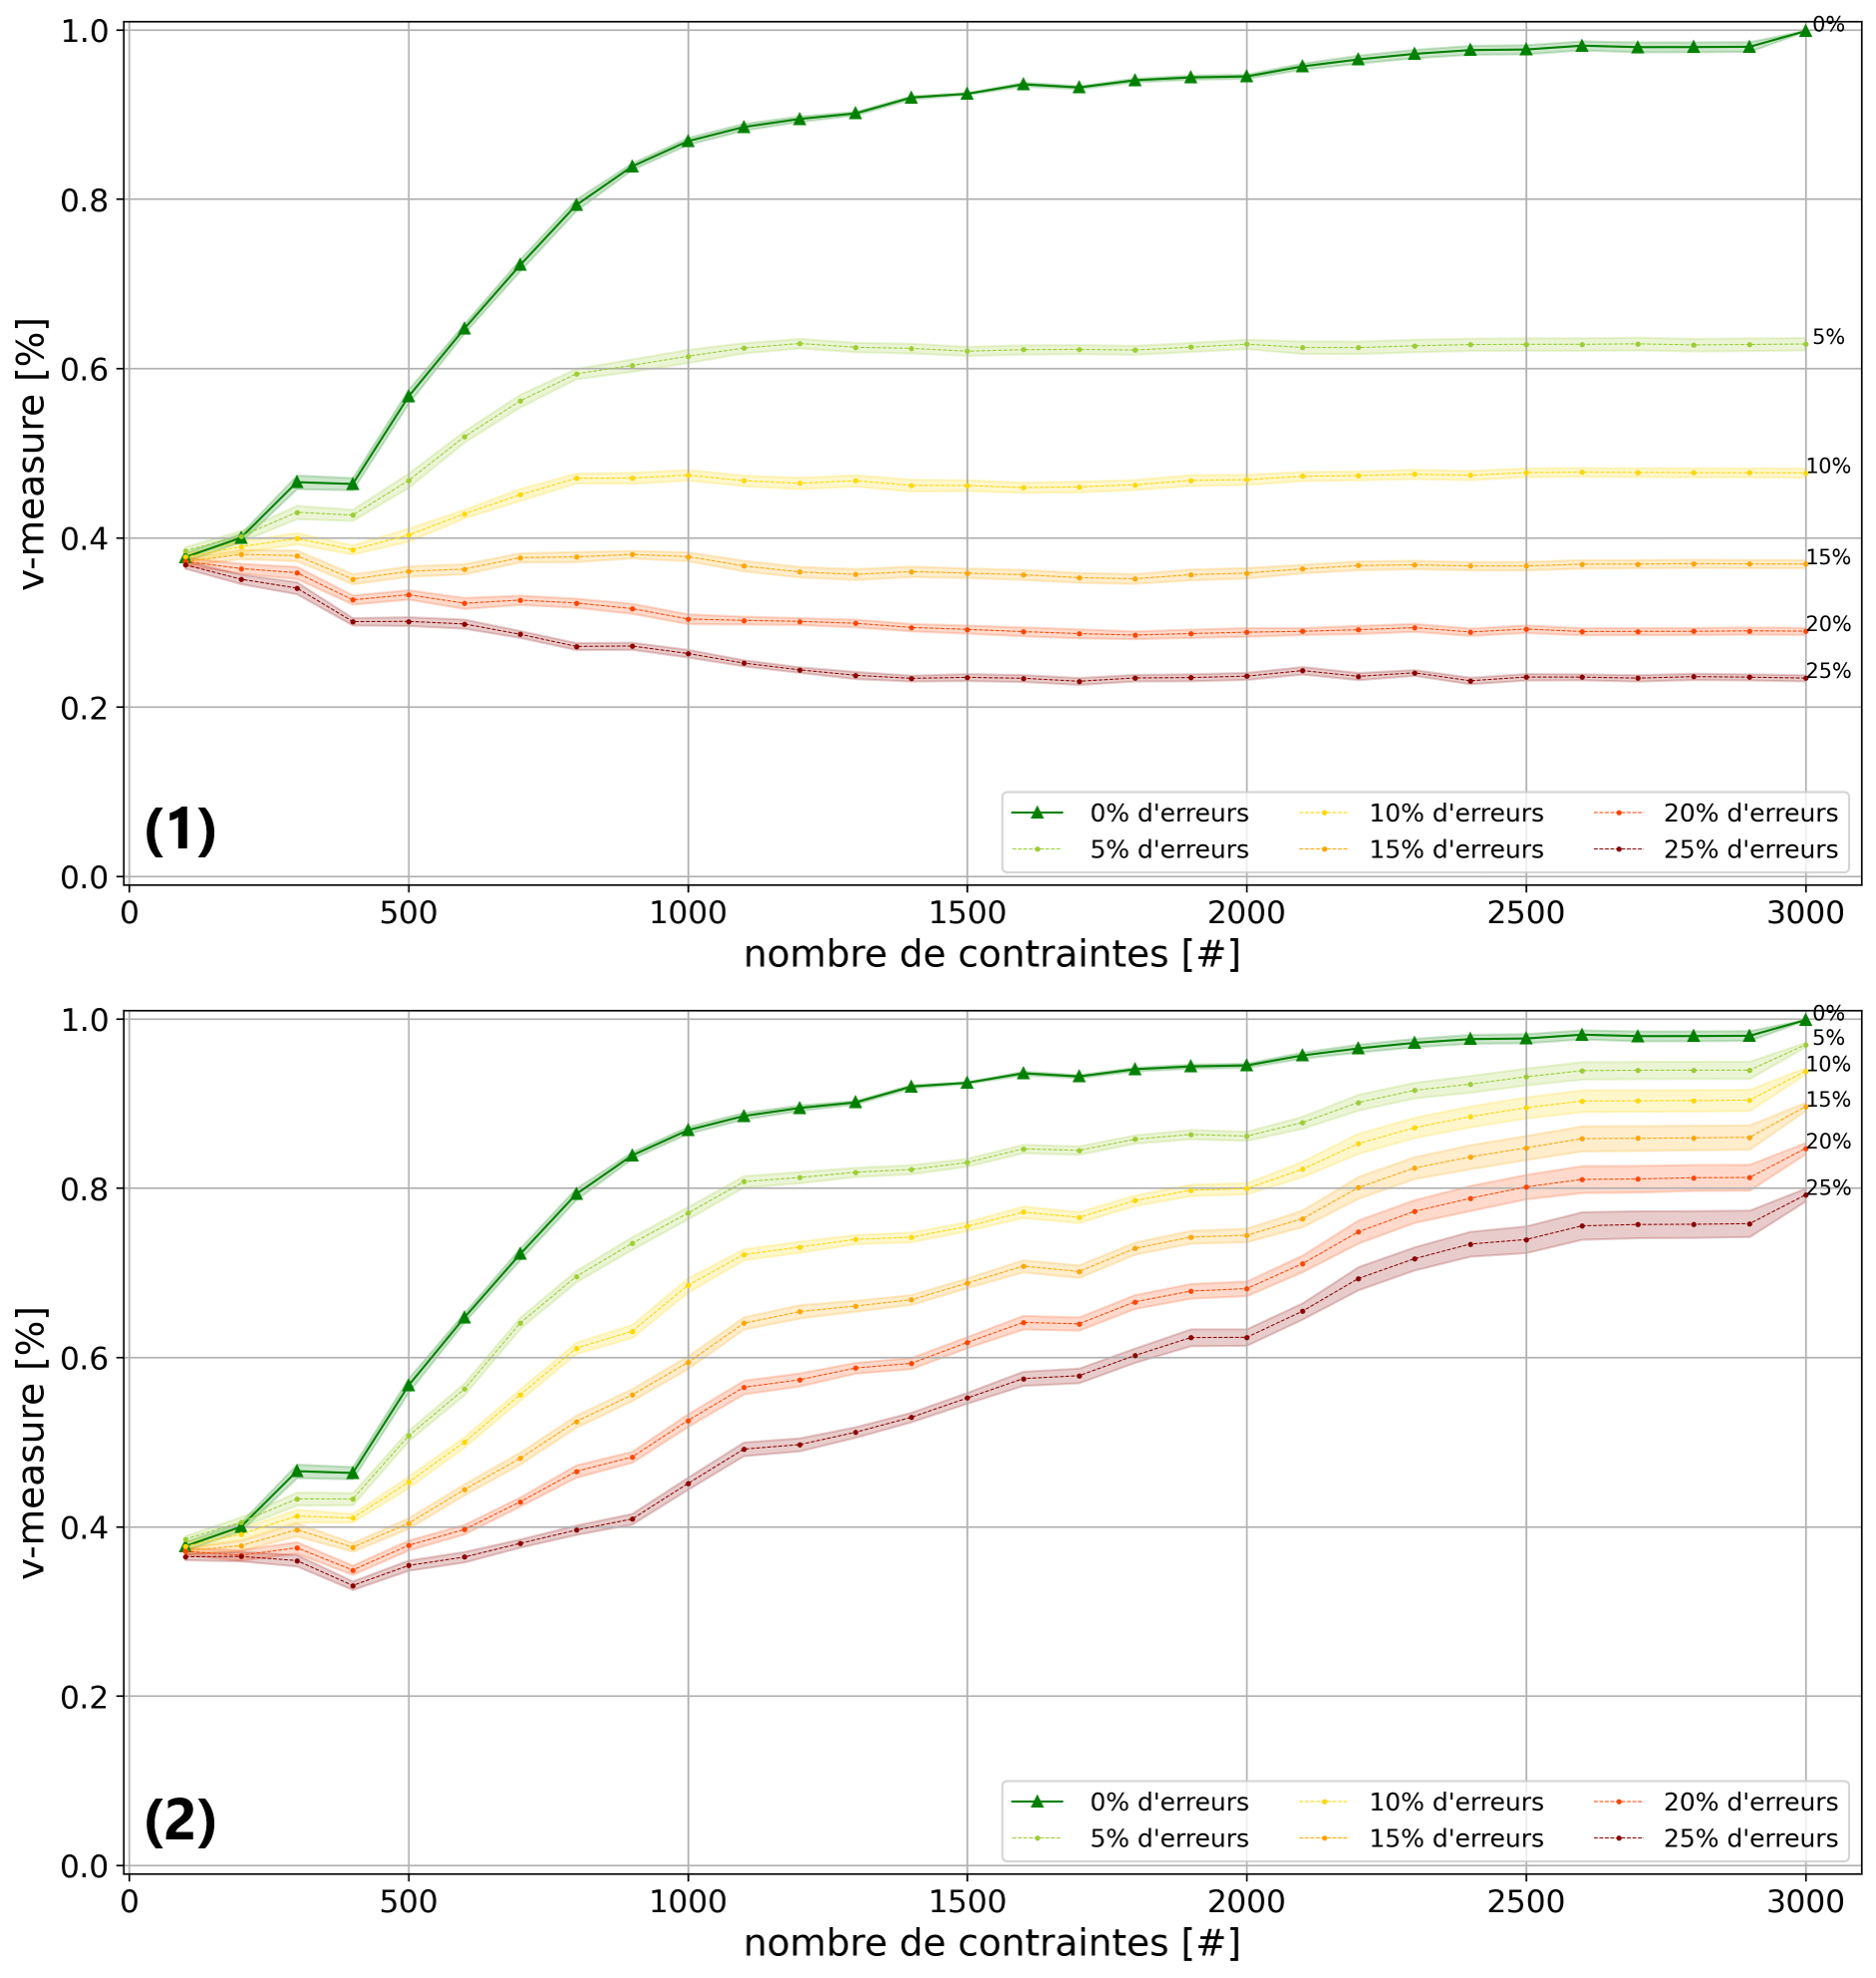
\includegraphics[width=0.95\textwidth]{figures/etude-robustesse-erreurs-et-corrections-closest}
				\caption{
					Évolution des similitudes moyennes (calculées en terme de \texttt{v-measure}) des résultats de \textit{clustering} des tentatives introduisant des erreurs d'annotation par rapport à la vérité terrain au cours des itérations.
					Les dégradés de couleurs des courbes représentent les déclinaisons de ces évolutions en fonction des différents taux d'annotations erronées (allant de $0$\% et $25$\%).
					\textbf{(1)} représente l'approche naïve ignorant les conflits d'annotation
					et \textbf{(2)} représente l'approche corrigeant les conflits détectés par le gestionnaire de contraintes.
					Toutes les courbes sont tronquées à $3~000$ contraintes (nombre maximum de contraintes nécessaire à une tentatives n'introduisant pas erreurs pour converger vers la vérité terrain).
				}
				\label{figure:4.6.2-ETUDE-ROBUSTESSE-ERREURS-ANNOTATION-ET-CORRECTION}
			\end{figure}
			
			% Description de la figure: cas naïf.
			Tout d'abord, observons l'approche \textit{naïve}, ignorant simplement les conflits (voir \textsc{Figure~\ref{figure:4.6.2-ETUDE-ROBUSTESSE-ERREURS-ANNOTATION-ET-CORRECTION}} \textbf{(1)}).
			Nous pouvons constater que les performances (basées sur la vérité terrain) plafonnent très rapidement si des incohérences sont introduites : dès $5$\% d'erreurs, le score de \texttt{v-measure} stagne autour de $65$\% à partir de $1~000$ contraintes, alors qu'une performance théorique d'environ $90$\% serait attendue pour une tentative idéale n'introduisant pas d'erreurs.
			D'autre part, si le taux de contraintes erronées est supérieur à $15$\%, nous pouvons remarquer que ces performances diminuent avant de stagner à des valeurs inférieures à $40$\% de \texttt{v-measure}.
			Pour finir sur cette première approche, tout porte à croire que ces faibles seuils performances perdurent au delà des $3~000$ contraintes (figure tronquée) : les tentatives s'éloignent donc significativement de la vérité terrain si des incohérences d'annotation sont insérées.
			
			% Description de la figure: cas correctif.
			Observons désormais l'approche \textit{avec correction}, ré-évaluant les contraintes lorsqu'un conflit est détecté par le gestionnaire de contraintes (voir \textsc{Figure~\ref{figure:4.6.2-ETUDE-ROBUSTESSE-ERREURS-ANNOTATION-ET-CORRECTION}} \textbf{(2)}).
			Nous pouvons constater que les tentatives introduisant des contraintes erronées subissent aussi un retard de performances, mais celui-ci est bien plus faible que celui encaissé par les approches naïves.
			Nous observons que toutes les courbes restent globalement croissantes, bien que le score moyen de $90$\% de \texttt{v-measure} par rapport à la vérité terrain n'est pas atteint en moins de $3~000$ contraintes par les tentatives ayant un taux d'erreurs supérieur à $15$\%.
			Nous pouvons toutefois espérer que cette convergence se poursuit au delà des $3~000$ contraintes (figure tronquée).
		
		%%% Discussion
		\subsubsection{Discussion}
		
			% Rappel de l'objectif : Intérêt de la correction en cas d'incohérences.
			L'objectif de cette étude est l'analyse de l'impact des différences de comportements intra-annotateur sur les résultats de notre méthode, plus particulièrement l'intérêt de corriger les incohérences d'annotations lorsqu'elles sont détectées par le gestionnaire de contraintes.
			Pour cela, nous avons comparé deux approches : une approche naïve ignorant simplement les conflits, et une deuxième approche les corrigeant lorsque ces derniers sont détectées.
		
			% Analyse : Super important de corriger !
			D'après l'analyse de la \textsc{Figure~\ref{figure:4.6.2-ETUDE-ROBUSTESSE-ERREURS-ANNOTATION-ET-CORRECTION}}, nous pouvons clairement déduire que l'absence de correction des incohérences pénalise significativement la méthode.
			En effet, sur le jeu de données utilisé comme vérité terrain, nous constatons une perte irréversible d'au moins $35$\% de \texttt{v-measure} dès l'introduction de $5$\% d'erreurs d'annotation, caractérisant ainsi une dérive importante des résultats si les conflits d'annotations ne sont pas corrigés.
			Toutefois, la mise en oeuvre d'un mécanisme simple de correction semble estomper en partie ces régressions de performances et permet à certaines tentatives introduisant des erreurs de rester compétitives
			(\textit{toutes les tentatives peuvent espérer atteindre $80$\% de \texttt{v-measure} en corrigeant leurs incohérences, alors que l'approche naïve les condamnait à une \texttt{v-measure} plafonnée}).
			Nous pouvons donc assurément conclure en faveur de la \textbf{nécessité de vérifier la base de contraintes et de corriger toute incohérence s'y trouvant}.
			
			% Remarque : En accord avec les approches incrémentale.
			Une telle conclusion confirme la sensibilité aux erreurs de cette approche incrémentale : si une erreur apparaît, elle peut rapidement se propager et impacter les résultats de la méthode.
			Dans notre cas, nous avons optimisé l'implémentation de notre \texttt{Clustering Interactif} pour obtenir un corpus d'apprentissage pertinent en un minimum d'annotation de contraintes.
			Or obtenir un nombre minimal implique de limiter la redondance parmi les contraintes annotées.
			De ce fait, certaines incohérences mal placées peuvent fortement influencer la base de contraintes et ainsi faire diverger les résultats.
			
			% Solution: Ajouter de la redondance.
			Pour contrer ce problème, nous avons deux pistes pouvant être explorées :
			
			\begin{itemize}
				% Introduction de redondance d'annotation.
				\item \textbf{introduire intentionnellement de la redondances} dans la base de contraintes annotées à l'aide d'une nouvelle méthode d'échantillonnage : ce moyen tire parti des propriétés de transitivité du graphe de contraintes pour identifier d'éventuelles incohérences d'annotation isolée ou masquée.
				Cette piste a cependant le désavantage d'ajouter de nouvelles contraintes peu informatives dans le simple but de mieux détecter certaines incohérences, introduisant donc un léger coût supplémentaire pour l'annotateur ;
				% Confronter la vision des annotateurs.
				\item \textbf{confronter plusieurs des annotateurs} sur les mêmes contraintes : en faisant annoter les mêmes contraintes par deux opérateurs différents, les erreurs d'annotation peuvent être révélées.
				Cette piste engendre aussi un surcoût car elle nécessite d'embaucher plusieurs annotateurs.
			\end{itemize}
			
			% Conclusion : choix entre rapidité ou qualité.
			\begin{leftBarAuthorOpinion}
				Dans les deux cas, il y a un choix à faire : \textbf{veut-on privilégier la qualité} (\textit{ajouter de la redondance et une double vérification, au prix d'un surcoût d'annotation}) \textbf{ou la rapidité de conception} (\textit{optimiser l'annotation pour une convergence en un minimum de contraintes, au risque d'introduire des incohérences dans la modélisation}) \textbf{?}
			\end{leftBarAuthorOpinion}
		
	%%%
	%%% Subsection 4.6.3: Étude de l'impact de la subjectivité de l'annotation sur la divergence des résultats obtenus
	%%%
	\subsection{Étude de l'impact de la subjectivité de l'annotation sur la divergence des résultats obtenus}
	\label{section:4.6.3-ETUDE-ROBUSTESSE-SUBJECTIVITE-ANNOTATION-ET-DIVERGENCE}
		
		% Introduction : différences entre intra- et inter-annotateurs.
		Dans la section précédente, nous nous sommes intéressés aux différences de comportement intra-annotateur et aux pistes permettant de limiter les erreurs d'annotation d'un seul opérateur.
		Cependant, nous devons aussi nous intéresser aux \textbf{différences inter-annotateurs} :
		en effet, nous avons pu voir en \textsc{Section~\ref{section:2.3.3.A-DEFIS-ANNOTATION-ASPECT-HUMAIN-INTER-ANNOTATEURS}} que la labellisation est une tâche subjective, et que la complexité du phénomène à modéliser ainsi que la diversité de profils d'annotateurs peuvent introduire des différences d'annotation.
		Mais ces différences ne sont pas synonymes d'erreurs, elles peuvent aussi être les témoins de \textbf{différences d'opinion entre les experts}.
		%
		\begin{leftBarAuthorOpinion}
			Pour aller plus loin, il est même mal avisé de parler d'\textit{erreurs} d'annotation car cela suppose qu'une comparaison avec une vérité terrain soit possible.
			Or, en situation réelle, cette vérité terrain est précisément en cours de construction à l'aide de notre méthodologie de \texttt{Clustering Interactif} : l'expert est responsable de la vision qu'il veut appliquer aux données durant son annotation, il est donc difficile de parler d'erreurs sans porter de jugement sur sa vision.
			Il convient donc mieux de parler de \textit{différences} d'annotation si deux experts ont une divergence de point de vue sur une donnée à annoter.
		\end{leftBarAuthorOpinion}
		
		% Objectif de l'expérience.
		Dans cette dernière étude, nous allons donc estimer la robustesse du \texttt{Clustering Interactif} en nous intéressant plus particulièrement aux différences d'annotation entre deux opérateurs.
		Pour cela, nous allons simuler de telles différences entre deux annotateurs fictifs : le premier sera représenté par la vérité terrain, et le second sera simulé en introduisant un certain taux de désaccords d'annotation à chaque itération.
		Nous discutons ensuite de l'écart de similarité entre les résultats de \textit{clustering} obtenus lorsque l'annotateur de référence atteint le seuil d'annotation partielle de son jeu de données (\textit{accord théorique de $90$\% de \texttt{v-measure} sur la vérité terrain qu'il recherche})
		Nous réalisons cette analyse sur des jeux de données de différentes tailles et pour plusieurs taux de désaccords insérées.
	
		%%% Protocole expérimental.
		\subsubsection{Protocole expérimental}
			
			% Pseudo-code.
			Pour résumer le protocole expérimental que nous décrivons ci-dessous, vous pouvez vous référer au pseudo-code décrit dans \textsc{Algorithme~\ref{algorithm:4.6.3-ETUDE-ROBUSTESSE-SUBJECTIVITE-ANNOTATION-ET-DIVERGENCE-PROTOCOLE}}.
			
			\begin{algorithm}
				\KwData{jeux de données annotées (vérités terrains) de tailles différentes}
				\KwIn{liste de taux de désaccords à insérer}
				%
				\ForEach{jeux de données à tester et taux de désaccords à insérer}{
					\textbf{initialisation (données)}: récupérer les données et la vérité terrain \;
					\textbf{initialisation (contraintes)}: créer une liste vide de contraintes \;
					\textbf{prétraitements}: supprimer le bruit dans les données avec \texttt{prep.simple} \;
					\textbf{vectorisation}: transformer les données en vecteurs avec \texttt{vect.tfidf} \;
					\textbf{clustering initial}: regrouper les données par similarité avec \texttt{clust.kmeans.cop} \;
					\textbf{évaluation}: estimer l'équivalence entre le \textit{clustering} et la vérité terrain \;
					\Repeat{annotation de toutes les contraintes possibles}{
						\textbf{échantillonnage}: sélectionner des contraintes avec \texttt{samp.closest.diff} \;
						\textbf{choix des désaccords}: définir les contraintes erronées \;
						\textbf{simulation d'annotation}: déterminer les contraintes avec la vérité terrain \;
						\textbf{intégration corrective}: ajouter les nouvelles contraintes au gestionnaire de contraintes, et ré-annoter les annotations en conflit \;
						\textbf{clustering}: regrouper les données par similarité avec \texttt{clust.kmeans.cop} \;
						\textbf{évaluation}: estimer l'équivalence entre le \textit{clustering} et la vérité terrain \;
					}
					\textbf{analyse locale}: afficher l'évolution de la similarité entre les \textit{clustering} de la tentative courante et les \textit{clustering} de la tentative de référence (n'ayant pas de différence d'annotation par rapport à la vérité terrain) \;
				}
				\textbf{analyse générale}: analyse des différences de résultats de \textit{clustering} obtenus par taille de jeux de données et par taux de désaccords insérés \;
				%
				\KwResult{discussion sur l'impact de la subjectivité de l'annotation sur la divergence des résultats de \textit{clustering} obtenu}
				%
				\caption{\textit{
					Description en pseudo-code du protocole expérimental de l'impact de la subjectivité de l'annotation sur la divergence des résultats.
				}}
				\label{algorithm:4.6.3-ETUDE-ROBUSTESSE-SUBJECTIVITE-ANNOTATION-ET-DIVERGENCE-PROTOCOLE}
			\end{algorithm}
			
			% Détails de l'expérience.
			\begin{leftBarInformation}
				Nous reprenons dans les grandes lignes le protocole expérimental de la précédente étude sur l'impact des erreurs d'annotations et l'intérêt de les corriger (voir \textsc{Section~\ref{section:4.6.2-ETUDE-ROBUSTESSE-ERREURS-ANNOTATION-ET-CORRECTION}}.
				Cependant, nous utilisons ici la vérité terrain pour représenter un opérateur de référence, et nous représentons le second opérateur par les différences d'annotation introduites. 
			\end{leftBarInformation}
			
			% Description des jeux de données.
			Nous utilisons cette fois deux vérités terrains comme références, représentant un \textbf{annotateur de référence} (\textit{et sa propre vision métier}) :
			\begin{itemize}
				\item le jeu de données \texttt{Bank Cards (v2.0.0)} : ce dernier traite des demandes les plus fréquentes des clients en ce qui concerne la gestion de leur carte bancaire.
				Il est composé de $1~000$ questions rédigées en français et réparties en $10$ classes (\texttt{perte ou vol de carte}, \texttt{carte avalée}, \texttt{commande de carte}, ...).
				Pour plus de détails, consultez l'\textsc{Annexe~\ref{annex:A.1-DATASET-BANK-CARDS}} ;
				\item le jeu de données \texttt{MLSUM FR Train Subset (v1.0.0-schild)} : ce dernier concerne les titres d'articles de journaux issus des catégories de publication les plus communes.
				Il est composé de $744$  titres d'articles rédigés et répartis en $14$ classes (\textit{économie}, \textit{sport}, ...).
				Pour plus de détails, consultez l'\textsc{Annexe~\ref{annex:A.2-DATASET-MLSUM-SUBSET-SCHILD}} ;
			\end{itemize}
			
			Pour utiliser facilement plusieurs jeux de données de tailles différentes tout en maîtrisant leur contenu, nous avons donc dupliqué aléatoirement des données issues de ces jeux de référence en y insérant des fautes de frappes.
			La taille des jeux de données générés varie entre $1~000$ à $5~000$ par pas de $500$.
			Il y a donc $9$ variations de chaque jeu de références, soit $18$ jeux utilisés de tailles différentes.
			
			% Remarque.
			\begin{leftBarWarning}
				Dans le cadre de cette étude, nous faisons l'hypothèse que cette création artificielle de données n'a pas d'impact majeur sur le nombre de contraintes nécessaires pour converger vers une vérité terrain.
			\end{leftBarWarning}
			
			% Description des tentatives de la méthode avec simulation d'erreurs.
			Sur ces jeux de données, nous exécutons une tentative complète\footnote{
				Tentative complète : itérations d'échantillonnage, d'annotation et de \textit{clustering} jusqu'à annotation de toutes les contraintes possibles.
			}
			de la méthode du \texttt{Clustering Interactif} en utilisant notre paramétrage favori \footnote{
				Paramétrage favori (atteindre $90$\% de \texttt{v-measure} avec un coût minimal): prétraitements simples (\texttt{prep.simple}), vectorisation \texttt{TF-IDF} (\texttt{vect.tfidf}), \textit{clustering} \texttt{KMeans} avec modèle \texttt{COP} (\texttt{clust.kmeans.cop}) et échantillonnage des données les plus proches dans des clusters différents (\texttt{sampl.closest.diff}).
			} (voir \textsc{Section~\ref{section:4.3-HYPOTHESE-COUTS}}).
			À nouveau, nous allons ajouter un pourcentage de contraintes erronées à chaque itération, représentant un \textbf{autre annotateur} (\textit{et sa propre vision métier du problème à modéliser}) :
			\begin{itemize}
				\item Le taux de désaccords insérés, variant de $0$\% à $25$\% \footnote{
					Choix de $0$\% à $25$\% : nous utilisons ici les estimations grossières de bornes maximale d'erreurs réalisées en \textsc{Section~\ref{section:4.6.1-ETUDE-ROBUSTESSE-SCORE-ACCORD}}.
				} par pas de $5$\%, reste fixe tout au long d'une même tentative de notre méthode : nous pouvons ainsi analyser l'impact d'un taux de désaccords fixe sur les résultats au courant des itérations ;
				\item Les contraintes divergentes à insérer sont tirées aléatoirement parmi le lot de contraintes qui aurait été échantillonné au cours d'une tentative sans introduction de différences : ainsi, nous pouvons comparer itération par itération toutes ces simulations car elles partagent la même base de contraintes (aux valeurs de \texttt{MUST-LINK} et \texttt{CANNOT-LINK} près) ;
			\end{itemize}
			
			% Description des tentatives de la méthode avec gestion des conflits.
			Puisque nous introduisons des différences d'annotations, des conflits peuvent apparaître dans le gestionnaire de contraintes.
			Pour rappel, un conflit est détecté dans le cas où l'ajout d'une nouvelle contrainte annotée contredit ce qui a été précédemment déduit grâce aux propriétés de transitivité des contraintes de types \texttt{MUST-LINK} et \texttt{CANNOT-LINK} (voir \textsc{Figure~\ref{figure:C.1.2-DESCRIPTION-IMPLEMENTATION-INTERACTIVE-CLUSTERING-CONTRAINTES-TRANSITIVITE}} en \textsc{Annexe~\ref{annex:C.1.2-DESCRIPTION-IMPLEMENTATION-INTERACTIVE-CLUSTERING-GESTION-DES-CONTRAINTES}}).
			En tirant parti des conclusion de la précédente étude, nous choisissons de corriger ces désaccords dès leur détection, et supposant que le second annotateur se range à la vision de l'annotateur de référence.
			Pour simuler cette correction réalisée par les experts, nous recréons à chaque itération le gestionnaire de contraintes en intégrant d'abord les contraintes correctes puis les contraintes divergentes ; ainsi, les conflits ne peuvent arriver qu'à l'ajout d'une contrainte divergente, et il suffit d'ajouter sa version exacte pour simuler la correction des experts.
			
			% Description des tentatives de la méthode avec les répétitions.
			Ainsi, il y a donc $6$ taux de désaccords, et chacune de ces simulations de désaccords seront répétées $2$ fois sur chaque tentative complète de la méthode pour limiter au mieux les aléas statistiques des tirages de contraintes divergentes, ce qui représente $12$ simulations par tentatives.
			Enfin, chaque tentative complète de \texttt{Clustering Interactif} est répétée $2$ fois pour limiter au mieux les aléas statistiques des exécutions, soit un nombre de $24$ tentatives complètes pour chacun des $18$ jeux de données, ce qui représente un total de $432$ tentatives à simuler au cours de cette expérience.
			
			% Description de l'analyse.
			Nous réalisons ensuite l'analyse des différences de résultats obtenu en estimant la similarité des \textit{clustering} entre une tentative introduisant des différences et sa tentative de référence n'en introduisant pas.
			Pour cela, nous procédons en trois temps :
			\begin{itemize}
				% Estimer le nombre de contraintes.
				\item nous estimons d'abord, pour chaque taille de jeu de données, le nombre moyen de contraintes nécessaires aux tentatives de référence pour atteindre un score de $90$\% de \texttt{v-measure} par rapport à leur vérité terrain ;
				% Retenir la vmeasure pour ce nombre de contraintes.
				\item nous estimons ensuite, pour chaque tentative introduisant des différences d'annotation, le score de \texttt{v-measure} entre leur résultat de \textit{clustering} et le résultat de \textit{clustering} de leur tentative de référence pour le nombre de contraintes déterminé précédemment (celui nécessaire à la tentative de référence pour atteindre un score de $90$\% par rapport à sa vérité terrain) ;
				% Comparer l'écart.
				\item enfin, nous discutons de ces scores moyens pour les différentes tailles de jeu de données et les différents taux de désaccords introduits.
			\end{itemize}
			Un exemple est illustré avec la \textsc{Figure~\ref{figure:4.6.3-ETUDE-ROBUSTESSE-SUBJECTIVITE-ANNOTATION-ET-DIVERGENCE-5000}}.
			
			% Note de l'auteur sur le choix du nombre de contraintes.
			\setcounter{localCounterOfFootnoteValue}{\value{footnote}}
			\begin{leftBarAuthorOpinion}
				Il est à noter que nous aurions pu estimer ce nombre de contraintes grâce à l'\textsc{Équation~\ref{equation:4.3.3-ETUDE-COUT-NOMBRE-CONTRAINTES}} \footnotemark, mais comme cette estimation théorique est une moyenne qui aurait pu décaler légèrement nos résultats.
				Nous avons donc préféré mesurer directement le nombre exact de contraintes nécessaires pour chaque tentative afin de ne pas avoir à analyser une double moyenne.
			\end{leftBarAuthorOpinion}
			% Rattraper les footnote.
				\stepcounter{localCounterOfFootnoteValue}
				\footnotetext[\value{localCounterOfFootnoteValue}]{
					\textsc{Équation~\ref{equation:4.3.3-ETUDE-COUT-NOMBRE-CONTRAINTES}}: $\texttt{constraints\_needed}~\propto~3.15 \cdot \texttt{dataset\_size}$
				}
			
			% Remarque sur le faible nombre de redondances des tentatives.
			\begin{leftBarWarning}
				Ces simulations étant plus lourdes que les précédentes, et en considérant le manque de temps pour réaliser cette étude, nous avons du diminuer le nombre de répétitions de nos tentatives ($1$ pour le génération des jeux de données, $2$ pour l'insertion des différences, $2$ pour l'exécution des tentatives complètes de la méthode).
				Les résultats obtenus nous permettent tout de même de discuter des tendances générales, mais il serait intéressant de compléter a posteriori les résultats de cette étude pour en améliorer la fiabilité.
			\end{leftBarWarning}
			
			% Référence scripts.
			\begin{leftBarReminder}
				Les scripts de l'expérience, réalisés avec des \textit{notebooks} \texttt{Python} (\cite{van-rossum-drake:2009:python-reference-manual}), sont disponibles dans un dossier dédié de \cite{schild:2021:cognitivefactory-interactiveclusteringcomparativestudy}.
				De plus, les jeux de données ainsi que les implémentations de notre \texttt{Clustering Interactif} sont détaillés respectivement en \textsc{Annexe~\ref{annex:A-ANNEXE-DATASET}} et en \textsc{Annexe~\ref{annex:C-ANNEXE-IMPLEMENTATIONS}}.
			\end{leftBarReminder}
		
		
		%%% Résultats
		\subsubsection{Résultats obtenus}
			
			% Exemple de résultat avec une figure à 5000 données.
			Commençons par un exemple de résultats pour un jeu de $5~000$ données.
			La \textsc{Figure~\ref{figure:4.6.3-ETUDE-ROBUSTESSE-SUBJECTIVITE-ANNOTATION-ET-DIVERGENCE-5000}} représente l'évolution moyenne de la \texttt{v-measure} du \textit{clustering} en fonction du nombre de contraintes annotées au cours des itérations de la méthode.
			Sur cette figure, la courbe ayant $0$\% de différence d'annotation représente l'évolution moyenne des tentatives de l'opérateur de référence : celles-ci convergent pas-à-pas vers la vérité terrain ($100$ de \texttt{v-measure}).
			Les autres courbes représentent les tentatives du second opérateur et la divergence de ses \textit{clustering} due à l'introduction de différence d'annotation.
			Dans un soucis de lisibilité, nous avons toutefois tronqué la figure à $50~000$ contraintes.

			% Figure d'exemple à 5000 données.
			\begin{figure}[!htb]
				\centering
				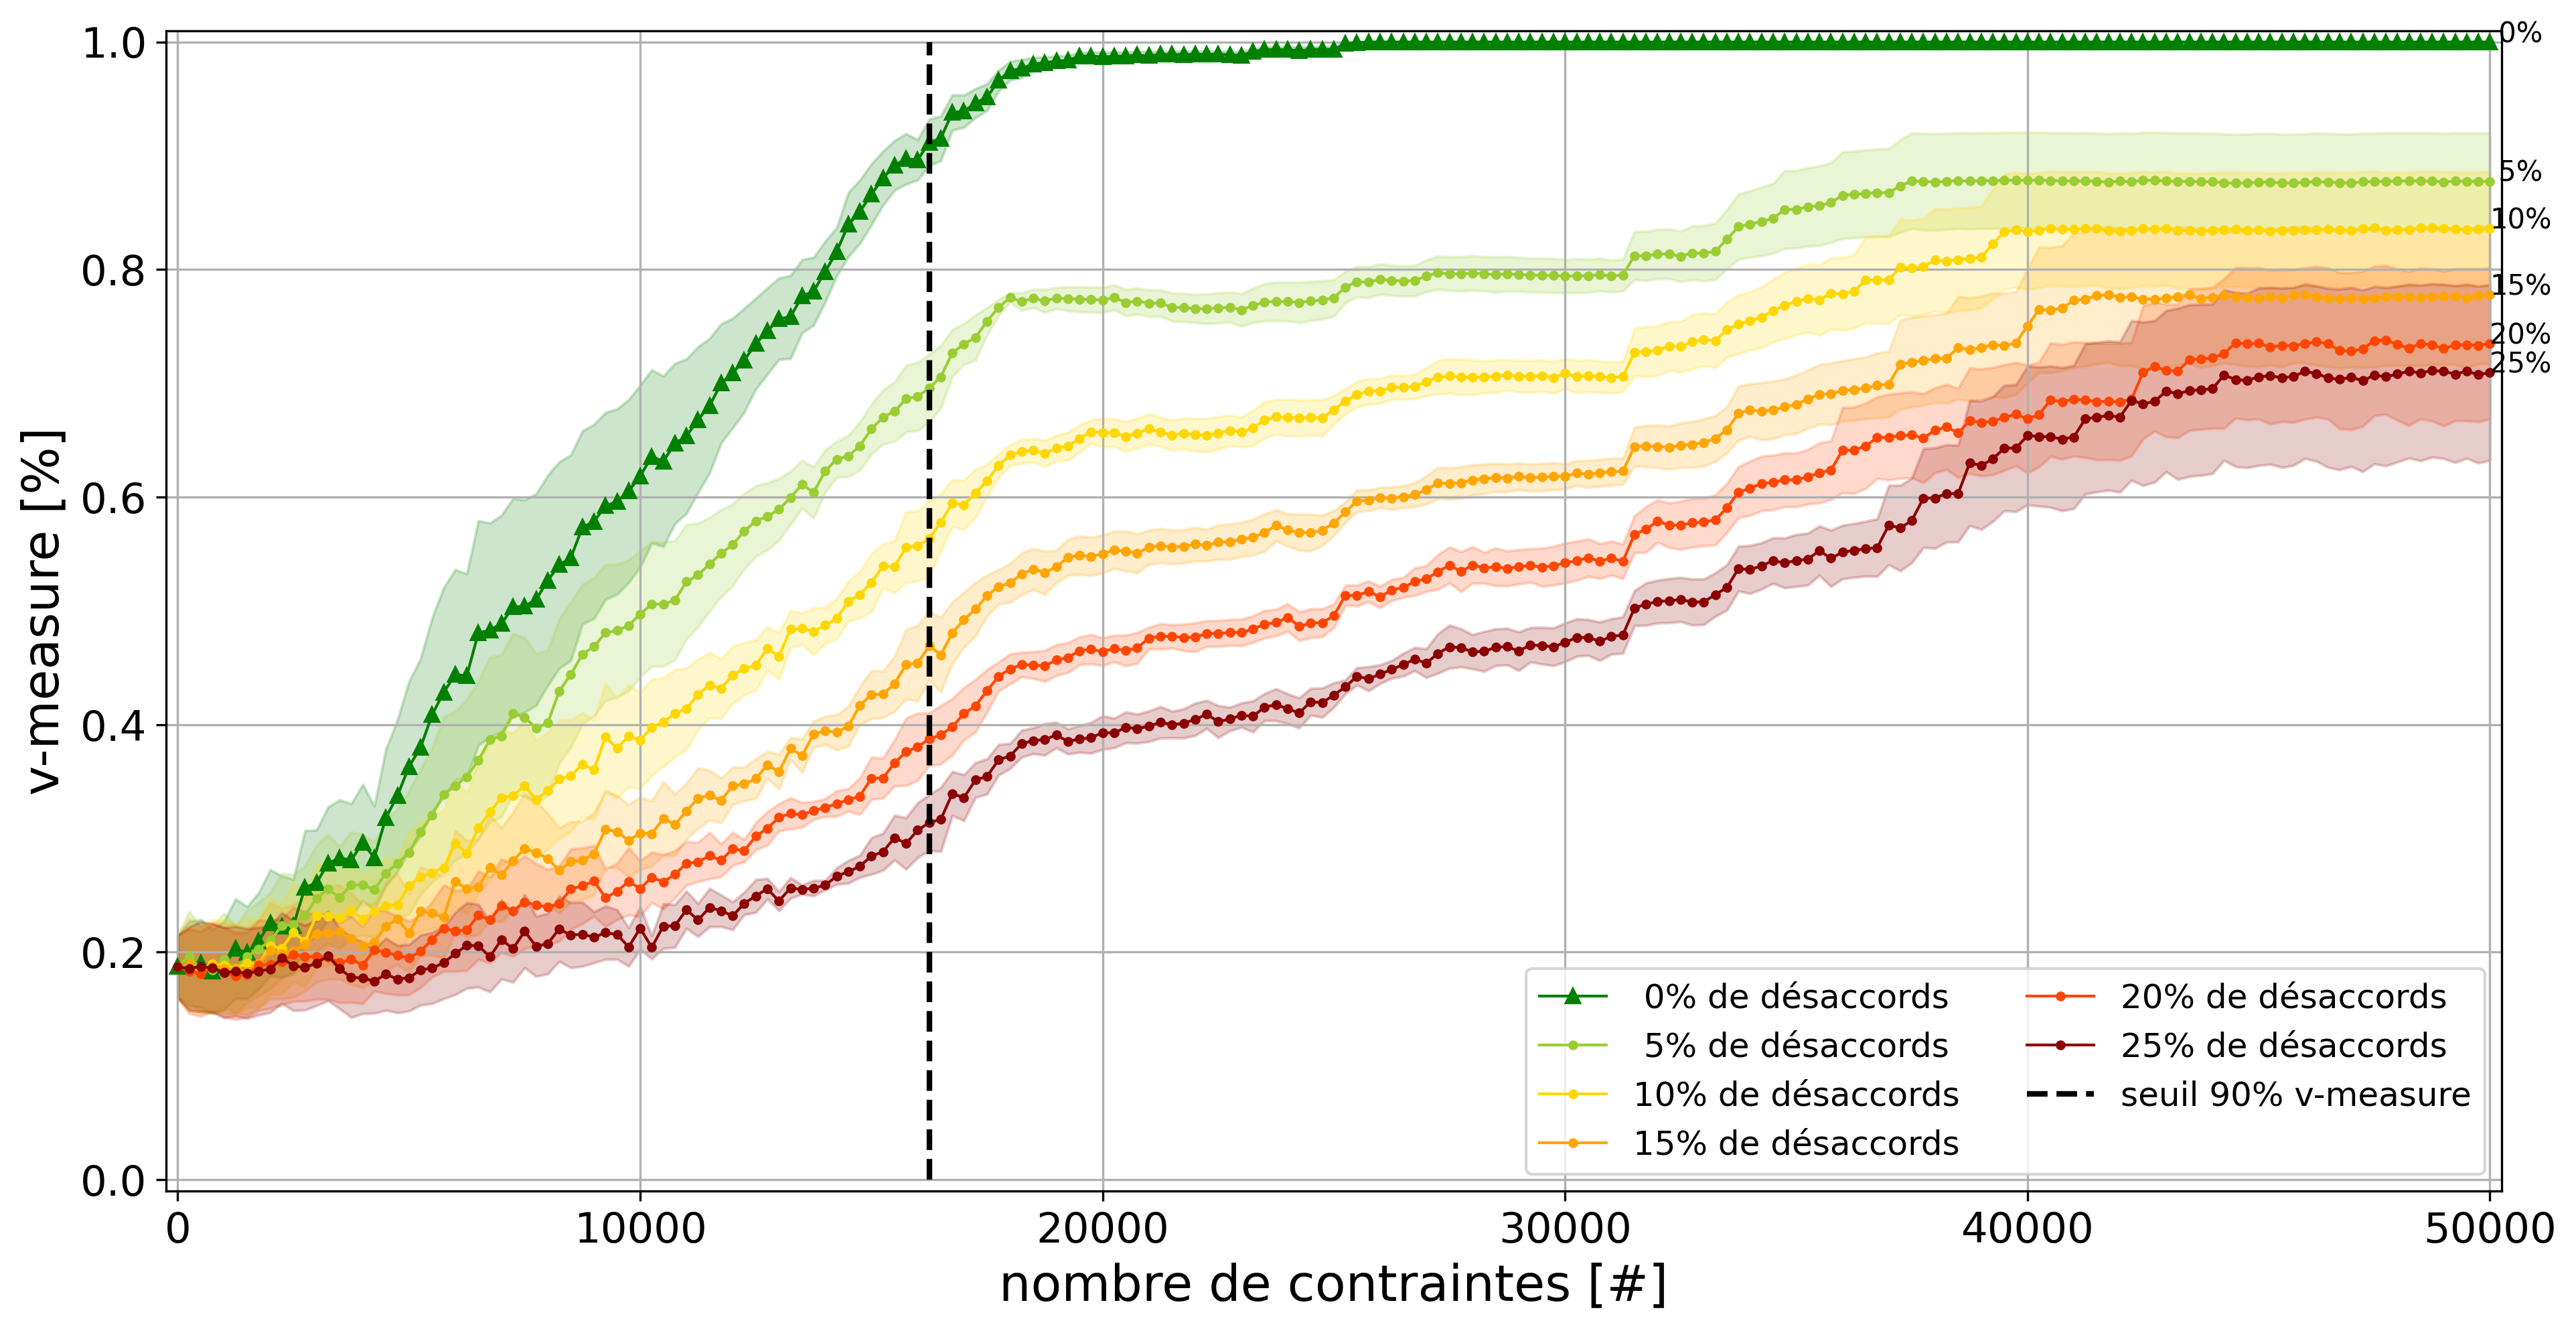
\includegraphics[width=0.95\textwidth]{figures/etude-robustesse-subjectivite-et-difference-5000}
				\caption{
					Exemple d'une évolution de similitudes moyennes (calculées en terme de \texttt{v-measure}) de résultats de \textit{clustering} de tentatives introduisant des différences d'annotation par rapport à la vérité terrain au cours des itérations, exemple pour une vérité terrain ayant une taille de $5~000$ données.
					Les dégradés de couleurs des courbes représentent les déclinaisons de ces évolutions en fonction des différents taux d'annotations divergentes (allant de $0$\% et $25$\%).
					La barre verticale indique le nombre moyen de contraintes nécessaires aux tentatives n'introduisant pas de désaccords pour obtenir un score de $90$\% de \texttt{v-measure} (\textit{ici: $16~250$ contraintes}).
				}
				\label{figure:4.6.3-ETUDE-ROBUSTESSE-SUBJECTIVITE-ANNOTATION-ET-DIVERGENCE-5000}
			\end{figure}
			
			% Analyse de la figure et lien vers la table.
			Grâce à cette figure, nous pouvons estimer à $16~250$ le nombre moyen de contraintes nécessaires aux tentatives de référence pour atteindre $90$\% de \texttt{v-measure} par rapport à la vérité terrain (\textit{ici: celle ayant $5~000$ données}).
			Sur cette base, nous pouvons identifier la similitude moyenne des résultats \textit{clustering} entre chaque tentative introduisant des désaccords et leur tentative de référence, calculée pour un nombre fixe de $16~250$ contraintes \footnote{
				Observation de $16~250$ contraintes nécessaires : lors d'une analyse théorique utilisant l'\textsc{Équation~\ref{equation:4.3.3-ETUDE-COUT-NOMBRE-CONTRAINTES}}, nous aurions estimé une moyenne de $3.15 \cdot 5~000~\propto~15~750$ contraintes, soit un écart de $500$ contraintes qui aurait introduit une légère variation dans nos résultats.
			}.
			Ces score de similitudes moyen sont rapportés dans la \textsc{Table~\ref{table:4.6.3-ETUDE-ROBUSTESSE-SUBJECTIVITE-ANNOTATION-ET-DIVERGENCE-CLUSTERING}}, chaque analyse pour une taille de jeu de données étant retranscrite dans une colonne dédiée.
			
			% Analyse du tableau de performance: chute drastique de performance.
			Nous pouvons constater les points suivants :
			\begin{itemize}
				% 
				\item la similarité est bien entendu de $100$\% pour un taux d'incohérence de $0$\% (\textit{une tentative de référence est comparée à elle-même}) ;
				% Taille fixe.
				\item à taille de jeu de données fixe, le taux de similarité diminue lorsque le taux de désaccords introduits augmentent ;
				l'amplitude de diminution varie environ entre $35$ points (\textit{pour une taille de $1~000$ données}) et $73$ points (\textit{pour une taille de $4~500$ données}).
				% Taux fixe.
				\item à un taux fixe de désaccords introduits, le taux de similitude diminue lorsque la taille du jeu de données augmentent ;
				l'amplitude de diminution varie environ entre $0$ points (\textit{pour l'introduction de $0$\% de désaccords}) et $33$ points (\textit{pour l'introduction de $25$\% de désaccords}).
			\end{itemize}
			
			% Table similitude avec \textit{clustering} sans erreurs.
			\begin{table}[!htb]
				% \small
				% \footnotesize
				\begin{center}
				\scalebox{0.8}{
					\begin{tabular}{|c|c||r|r|r|r|r|r|r|r|r|}
					
						\hhline{~~|---------}
						% ENTETE DU TABLEAU
						\multicolumn{2}{c|}{}
							& \multicolumn{9}{c|}{
								\cellcolor{colorTableHeader!15}
								\shortstack{Taille des jeux de données}
							}
							\tabularnewline
							\hhline{~~|-|-|-|-|-|-|-|-|-|}
						% Taille du jeu de données
						\multicolumn{2}{c|}{}
							& \cellcolor{colorTableHeader!15} $1~000$
							& \cellcolor{colorTableHeader!15} $1~500$
							& \cellcolor{colorTableHeader!15} $2~000$
							& \cellcolor{colorTableHeader!15} $2~500$
							& \cellcolor{colorTableHeader!15} $3~000$
							& \cellcolor{colorTableHeader!15} $3~500$
							& \cellcolor{colorTableHeader!15} $4~000$
							& \cellcolor{colorTableHeader!15} $4~500$
							& \cellcolor{colorTableHeader!15} $5~000$
							\tabularnewline
							\hhline{~|-|=|=|=|=|=|=|=|=|=|}
							
						% Contraintes annotées.
						\multicolumn{1}{c|}{}
							& \cellcolor{colorTableHeader!15} \textit{Contraintes}
							& \multirow{2}{*}{$4~250$}
							& \multirow{2}{*}{$6~000$}
							& \multirow{2}{*}{$7~250$}
							& \multirow{2}{*}{$8~750$}
							& \multirow{2}{*}{$10~250$}
							& \multirow{2}{*}{$11~250$}
							& \multirow{2}{*}{$12~250$}
							& \multirow{2}{*}{$13~500$}
							& \multirow{2}{*}{$16~250$}
							\tabularnewline
						\multicolumn{1}{c|}{}
							& \cellcolor{colorTableHeader!15} \textit{annotées}
							&
							&
							&
							&
							&
							&
							&
							&
							&
							\tabularnewline
							\hline
							
						% Erreur 0%
						\cellcolor{colorTableHeader!15}
							& \cellcolor{colorTableHeader!15}
							& $100.00$\%
							& $100.00$\%
							& $100.00$\%
							& $100.00$\%
							& $100.00$\%
							& $100.00$\%
							& $100.00$\%
							& $100.00$\%
							& $100.00$\%
							\tabularnewline
						\cellcolor{colorTableHeader!15}
							& \multirow{-2}{*}{
								\cellcolor{colorTableHeader!15}
								$0$\%
							}
							& \footnotesize $(\pm0.00)$
							& \footnotesize $(\pm0.00)$
							& \footnotesize $(\pm0.00)$
							& \footnotesize $(\pm0.00)$
							& \footnotesize $(\pm0.00)$
							& \footnotesize $(\pm0.00)$
							& \footnotesize $(\pm0.00)$
							& \footnotesize $(\pm0.00)$
							& \footnotesize $(\pm0.00)$
							\tabularnewline
							\hhline{~----------}
							
						% Erreur 0.05%
						\cellcolor{colorTableHeader!15}
							& \cellcolor{colorTableHeader!15}
							& $86.16$\%
							& $78.56$\%
							& $80.09$\%
							& $74.81$\%
							& $75.06$\%
							& $74.72$\%
							& $71.86$\%
							& $70.07$\%
							& $71.03$\%
							\tabularnewline
						\cellcolor{colorTableHeader!15}
							& \multirow{-2}{*}{
								\cellcolor{colorTableHeader!15}
								$5$\%
							}
							& \footnotesize $(\pm3.52)$
							& \footnotesize $(\pm1.50)$
							& \footnotesize $(\pm1.27)$
							& \footnotesize $(\pm1.62)$
							& \footnotesize $(\pm1.02)$
							& \footnotesize $(\pm1.84)$
							& \footnotesize $(\pm0.91)$
							& \footnotesize $(\pm1.29)$
							& \footnotesize $(\pm3.09)$
							\tabularnewline
							\hhline{~----------}
						
						% Erreur 0.10%
						\cellcolor{colorTableHeader!15}
							& \cellcolor{colorTableHeader!15}
							& $79.84$\%
							& $66.02$\%
							& $66.95$\%
							& $61.13$\%
							& $61.64$\%
							& $60.93$\%
							& $57.70$\%
							& $54.00$\%
							& $57.01$\%
							\tabularnewline
						\cellcolor{colorTableHeader!15}
							& \multirow{-2}{*}{
								\cellcolor{colorTableHeader!15}
								$10$\%
							}
							& \footnotesize $(\pm6.22)$
							& \footnotesize $(\pm2.00)$
							& \footnotesize $(\pm1.46)$
							& \footnotesize $(\pm1.55)$
							& \footnotesize $(\pm1.05)$
							& \footnotesize $(\pm1.92)$
							& \footnotesize $(\pm1.52)$
							& \footnotesize $(\pm1.84)$
							& \footnotesize $(\pm3.65)$
							\tabularnewline
							\hhline{~----------}
						
						% Erreur 0.15%
						\cellcolor{colorTableHeader!15}
							& \cellcolor{colorTableHeader!15}
							& $73.94$\%
							& $58.64$\%
							& $57.13$\%
							& $51.01$\%
							& $48.25$\%
							& $52.33$\%
							& $48.52$\%
							& $42.13$\%
							& $47.41$\%
							\tabularnewline
						\cellcolor{colorTableHeader!15}
							& \multirow{-2}{*}{
								\cellcolor{colorTableHeader!15}
								$15$\%
							}
							& \footnotesize $(\pm8.48)$
							& \footnotesize $(\pm2.21)$
							& \footnotesize $(\pm1.97)$
							& \footnotesize $(\pm1.43)$
							& \footnotesize $(\pm2.14)$
							& \footnotesize $(\pm2.04)$
							& \footnotesize $(\pm1.61)$
							& \footnotesize $(\pm1.43)$
							& \footnotesize $(\pm3.27)$
							\tabularnewline
							\hhline{~----------}
						
						% Erreur 0.20%
						\cellcolor{colorTableHeader!15}
							& \cellcolor{colorTableHeader!15}
							& $68.96$\%
							& $51.92$\%
							& $48.85$\%
							& $42.01$\%
							& $41.57$\%
							& $43.37$\%
							& $40.56$\%
							& $34.87$\%
							& $39.08$\%
							\tabularnewline
						\cellcolor{colorTableHeader!15}
							& \multirow{-2}{*}{
								\cellcolor{colorTableHeader!15}
								$20$\%
							}
							& \footnotesize $(\pm9.61)$
							& \footnotesize $(\pm2.30)$
							& \footnotesize $(\pm2.31)$
							& \footnotesize $(\pm0.96)$
							& \footnotesize $(\pm2.00)$
							& \footnotesize $(\pm1.71)$
							& \footnotesize $(\pm1.94)$
							& \footnotesize $(\pm1.15)$
							& \footnotesize $(\pm2.51)$
							\tabularnewline
							\hhline{~----------}
						
						% Erreur 0.25%
						\cellcolor{colorTableHeader!15}
							& \cellcolor{colorTableHeader!15}
							& $65.05$\%
							& $44.12$\%
							& $40.19$\%
							& $35.88$\%
							& $35.31$\%
							& $37.31$\%
							& $32.47$\%
							& $26.73$\%
							& $31.90$\%
							\tabularnewline
						\multirow{-12}{*}{
							\cellcolor{colorTableHeader!15}
							\rotatebox[origin=c]{90}{Taux de désaccords simulés}
						}
							& \multirow{-2}{*}{
								\cellcolor{colorTableHeader!15}
								$25$\%
							}
							& \footnotesize $(\pm10.78)$
							& \footnotesize $(\pm2.30)$
							& \footnotesize $(\pm2.01)$
							& \footnotesize $(\pm0.98)$
							& \footnotesize $(\pm1.25)$
							& \footnotesize $(\pm2.04)$
							& \footnotesize $(\pm1.46)$
							& \footnotesize $(\pm1.56)$
							& \footnotesize $(\pm2.56)$
							\tabularnewline
							\hline
						
					\end{tabular}
				}
				\end{center}
				\caption{
					Estimation de la \textbf{similitude moyenne} (calculée en terme de \texttt{v-measure}) des résultats de \textit{clustering} des tentatives introduisant des désaccords d'annotation \textbf{par rapport aux résultats de \textit{clustering} de leurs tentatives de référence}. \\
					Cette similitude est rapportée en fonction de la taille du jeu de données utilisé et du taux de désaccords introduits lors des tentatives.
					Pour chaque taille de jeu de données, les calculs sont réalisés avec un nombre de contraintes fixe, choisi comme étant le nombre de contraintes nécessaires à une tentative de référence pour atteidre une \texttt{v-measure} moyenne de $90$\% avec sa vérité terrain (ce nombre est rapporté en deuxième ligne).
				}
				\label{table:4.6.3-ETUDE-ROBUSTESSE-SUBJECTIVITE-ANNOTATION-ET-DIVERGENCE-CLUSTERING}
			\end{table}

		%%% Discussion
		\subsubsection{Discussion}
		
			% % Rappel de l'objectif : Impact de la subjectivité des annotateur sur la différence de \textit{clustering}.
			L'objectif de cette étude est l'analyse de l'impact des différences de comportements inter-annotateurs sur les résultats de notre méthode, plus particulièrement l'impact de la subjectivité des opérateurs manifestée par des désaccords d'annotation sur le résultat du \textit{clustering} obtenu.
			Pour cela, nous avons analysé l'évolution de la similarité en simulant des désaccords d'annotation pour plusieurs tailles de jeux de données.
			
			% Analyse : divergences importantes !
			Sur la base des résultats rapportés dans la \textsc{Table~\ref{table:4.6.3-ETUDE-ROBUSTESSE-SUBJECTIVITE-ANNOTATION-ET-DIVERGENCE-CLUSTERING}}, nous pouvons constater que les résultats de \textit{clustering} divergent rapidement si des désaccords d'annotation sont présents.
			En effet, l'introduction de $5$\% de différences fait diverger les résultats d'au moins $14$ points de \texttt{v-measure}, et cette divergence est plus forte lorsque la taille du jeu de données augmente.
			Si nous prenons le cas extrême ($25$\% de désaccord, taille de $4~500$ données), la similitude des \textit{clusterings} obtenus n'est en moyenne plus que de $26.73$\% au bout de $13~500$ contraintes.
			Nous pouvons donc conclure qu'en l'état, le \texttt{Clustering Interactif} est sensible à la subjectivité des annotateurs.
			
			% Remarque : En accord avec les approches incrémentale.
			Une telle conclusion est en accord avec le caractère incrémental de la méthode : une différence d'annotation peut rapidement se propager et faire diverger les résultats de la méthode.
			Dans notre cas, nous avons optimisé l'implémentation de notre \texttt{Clustering Interactif} pour obtenir un corpus d'apprentissage pertinent un minimum d'annotation de contraintes.
			Or cette notion de pertinence est subjective à la vision de l'expert annotant les données.
			De ce fait, si deux annotateurs ne sont pas d'accord sur la vision à appliquer aux données lors de l'annotation, il est normal de voir leurs résultats de \textit{clustering} diverger.
			Nous pourrions résumer cette situation par le fait que \textbf{ces deux experts ne recherchent pas la même vérité terrain, d'où la divergence significative de leurs résultats}.
			Ainsi, la sensibilité de notre méthode n'est pas la racine du problème, elle met plutôt en lumière le besoin de confronter les opinions des experts afin qu'ils puissent s'accorder.
			
			% Solution: Ajouter de la redondance !
			En nous basant sur notre revue de littérature (notamment la \textsc{Section~\ref{section:2.3.3.A-DEFIS-ANNOTATION-ASPECT-HUMAIN-INTER-ANNOTATEURS}}), nous conseillons à un projet d'annotation voulant utiliser notre implémentation du \texttt{Clustering Interactif} pour concevoir une base d'apprentissage d'\textbf{employer au moins $3$ opérateurs et de les confronter aux mêmes contraintes à chaque itération} de la méthode.
			Ainsi, si ces derniers ont des différences d'opinion sur la modélisation du problème, celles-ci se manifesteront en observant le score d'accord inter-annotateurs.
			Il conviendra alors d'organiser une session de débat pour ré-annoter les désaccords et décider des adaptations à prévoir dans le guide d'annotation du projet.
			%
			\begin{leftBarIdea}
				% Pour aider la résolution du conflit : observer le graphe de contraintes.
				Pour aider à trouver un accord lors de la revue, une prise de recul peut être nécessaire.
				Pour ce faire, les experts pourraient par exemple \textbf{observer le graphe de contraintes} déjà annotées.
				En effet, le gestionnaire de contraintes gère les propriétés de transitivité entre celle-ci, créant ainsi des composants connexes de données liées par les contraintes \texttt{MUST-LINK} et distinguées par les contraintes \texttt{CANNOT-LINK} (voir \textsc{Annexe~\ref{annex:C.1.2-DESCRIPTION-IMPLEMENTATION-INTERACTIVE-CLUSTERING-GESTION-DES-CONTRAINTES}}).
				Or le règlement d'un désaccord va nécessairement impacter ces composants connexes : en les rapprochant si le désaccord est tranché en faveur d'un \texttt{MUST-LINK}, en les éloignant sinon.
				Par conséquent, il serait intéressant d'aiguiller le débat pour anticiper les conséquences du consensus à trouver : ces composants sont-ils à rapprocher ? à distinguer ? ou sont-ils 
				éventuellement à remettre en question ?

				% Si toujours désaccord : laisser le \textit{clustering} trancher.
				Si malgré cette prise de recul, aucun accord n'a été trouvé, il est possible de ne pas caractériser cette contrainte et de \textbf{laisser l'algorithme de \textit{clustering} trancher le débat}.
				En effet, la philosophie de la méthode d'annotation basée sur le \texttt{Clustering Interactif} repose sur la coopération entre l'Homme et la machine : dans cette situation, il peut être intéressant de simplement observer quelle solution est proposée par la machine pour segmenter les données tout en respectant les autres contraintes déjà annotées.
			\end{leftBarIdea}
			
			% Problème : surcoût.
			Bien entendu, une telle approche engendre un coût supplémentaire aux estimations réalisées dans la \textsc{Section~\ref{section:4.3-HYPOTHESE-COUTS}} :
			\begin{itemize}
				\item d'une part, nous triplons la charge salariale à investir dans le but de redonder les contraintes annotées ;
				\item d'autre part, nous introduisons un délais supplémentaire en organisant des revues de désaccords de contraintes, du moins tant que des désaccords de visions subsistent.
			\end{itemize}
			% Mais ces surcoûts sont prévisibles ou bénéfiques.
			Néanmoins, ces surcoûts participent à l'amélioration de la stabilité de la base d'apprentissage en cours de construction.
			Par ailleurs, nous pouvons noter que :
			\begin{itemize}
				\item un projet d'annotation classique emploie aussi plusieurs opérateurs : ce surcoût correspond donc plutôt à un investissement supplémentaire au profit d'une fiabilisation de la qualité de ses résultats ;
				\item un projet d'annotation classique est déjà confronté au besoin d'organiser des sessions de revue de sa modélisation (voir l'étape \textit{Revise} du cycle \texttt{MATTER}) : l'avantage de notre méthode réside néanmoins sur la possibilité de discuter directement des divergences d'opinions en analysant des cas d'usage métier (\textit{évaluation d'une contrainte à l'aide de compétences métiers}) plutôt que de discuter de divergences d'opinions sur l'interprétation d'une abstraction du problème (\textit{remise en cause d'une modélisation à l'aide de compétences analytiques}).
			\end{itemize}
			
			% Conclusion : choix entre rapidité et qualité.
			\begin{leftBarAuthorOpinion}
				Nous concluons cette discussion par la même remarque faite à la fin de la précédente étude de robustesse : \textbf{il y a un choix à faire entre privilégier la qualité} (\textit{ajouter de la redondance pour clarifier les désaccords d'opinion, au prix d'un surcoût d'annotation}) \textbf{ou la rapidité de conception} (\textit{optimiser l'annotation pour une convergence en un minimum de contraintes, au risque d'introduire des incohérences dans la modélisation}).
			\end{leftBarAuthorOpinion}
	
	
	%%%
	%%% Subsection 4.6.4: Bilan concernant la robustesse du \texttt{Clustering Interactif}
	%%%
	\subsection{Bilan concernant la robustesse du \textit{Clustering Interactif}}
	\label{section:4.6.4-ETUDE-ROBUSTESSE-MISE-EN-COMMUN}
	
		% Conclusion.
		\begin{leftBarSummary}
			Au cours de cette étude de robustesse, nous avons pu voir que :
			\begin{itemize}
				% Sensible aux erreurs car optimisé.
				\item[\itemok] Le \texttt{Clustering Interactif}, comme tout autre approche incrémentale, est \textbf{sensible aux erreurs et aux désaccords d'annotation} : en effet, la méthode est optimisée pour converger vers une base d'apprentissage en un minimum de contraintes, donc toute différence d'annotation peut rapidement se propager ;
				% Solution intra-annotateur.
				\item[\itemok] Pour \textbf{combattre les erreurs d'annotations} (\textit{divergences intra-annotateur}), il peut être intéressant d'\textbf{ajouter de la redondance dans les annotations} : cela permet au gestionnaire de contraintes de vérifier les propriétés de transitivité des contraintes \texttt{MUST-LINK} et \texttt{CANNOT-LINK}, contribuant ainsi à la détection d'éventuelles incohérences ;
				% Solution inter-annotateurs.
				\item[\itemok] Pour \textbf{combattre les différences d'opinions} (\textit{désaccords inter-annotateurs}), il est nécessaire de \textbf{confronter plusieurs opérateurs sur les mêmes annotations contraintes} : cela permet de débattre des désaccords d'interprétation de cas d'usages métier dissimulés derrières les différences de labellisation, et de compléter le guide d'annotation si besoin ;
				% Choix entre qualité et rapidité.
				\item[\itemok] Il y a un choix à faire entre \textbf{privilégier la qualité} (\textit{vérification des annotations et harmonisation des opinions, au prix d'un surcoût d'annotation}) \textbf{ou la rapidité de conception} (\textit{optimisation de la convergence en un minimum d'annotation, au risque d'introduire des incohérences dans la modélisation}).
			\end{itemize}
		\end{leftBarSummary}